\documentclass[journal = esthag, manuscript = article]{achemso}\usepackage[]{graphicx}\usepackage[]{color}
%% maxwidth is the original width if it is less than linewidth
%% otherwise use linewidth (to make sure the graphics do not exceed the margin)
\makeatletter
\def\maxwidth{ %
  \ifdim\Gin@nat@width>\linewidth
    \linewidth
  \else
    \Gin@nat@width
  \fi
}
\makeatother

\definecolor{fgcolor}{rgb}{0.345, 0.345, 0.345}
\newcommand{\hlnum}[1]{\textcolor[rgb]{0.686,0.059,0.569}{#1}}%
\newcommand{\hlstr}[1]{\textcolor[rgb]{0.192,0.494,0.8}{#1}}%
\newcommand{\hlcom}[1]{\textcolor[rgb]{0.678,0.584,0.686}{\textit{#1}}}%
\newcommand{\hlopt}[1]{\textcolor[rgb]{0,0,0}{#1}}%
\newcommand{\hlstd}[1]{\textcolor[rgb]{0.345,0.345,0.345}{#1}}%
\newcommand{\hlkwa}[1]{\textcolor[rgb]{0.161,0.373,0.58}{\textbf{#1}}}%
\newcommand{\hlkwb}[1]{\textcolor[rgb]{0.69,0.353,0.396}{#1}}%
\newcommand{\hlkwc}[1]{\textcolor[rgb]{0.333,0.667,0.333}{#1}}%
\newcommand{\hlkwd}[1]{\textcolor[rgb]{0.737,0.353,0.396}{\textbf{#1}}}%
\let\hlipl\hlkwb

\usepackage{framed}
\makeatletter
\newenvironment{kframe}{%
 \def\at@end@of@kframe{}%
 \ifinner\ifhmode%
  \def\at@end@of@kframe{\end{minipage}}%
  \begin{minipage}{\columnwidth}%
 \fi\fi%
 \def\FrameCommand##1{\hskip\@totalleftmargin \hskip-\fboxsep
 \colorbox{shadecolor}{##1}\hskip-\fboxsep
     % There is no \\@totalrightmargin, so:
     \hskip-\linewidth \hskip-\@totalleftmargin \hskip\columnwidth}%
 \MakeFramed {\advance\hsize-\width
   \@totalleftmargin\z@ \linewidth\hsize
   \@setminipage}}%
 {\par\unskip\endMakeFramed%
 \at@end@of@kframe}
\makeatother

\definecolor{shadecolor}{rgb}{.97, .97, .97}
\definecolor{messagecolor}{rgb}{0, 0, 0}
\definecolor{warningcolor}{rgb}{1, 0, 1}
\definecolor{errorcolor}{rgb}{1, 0, 0}
\newenvironment{knitrout}{}{} % an empty environment to be redefined in TeX

\usepackage{alltt}

% \usepackage[version=3]{mhchem}
\usepackage[T1]{fontenc}
\usepackage[colorlinks  =true, allcolors=Blue]{hyperref}
\usepackage[usenames,dvipsnames]{xcolor}
\usepackage{lineno}
\usepackage{cleveref}
\usepackage{acronym}
\usepackage{paralist}
\usepackage{setspace}
\usepackage{showlabels}

% cleveref options
\crefname{table}{Table}{Tables}
\crefname{figure}{Figure}{Figures}
\renewcommand{\figurename}{Figure}

%acronyms
\acrodef{chla}[chl-\textit{a}]{chlorophyll \textit{a}}
\acrodef{din}[DIN]{dissolved inorganic nitrogen}
\acrodef{emp}[EMP]{Environmental Monitoring Program}
\acrodef{iep}[IEP]{Interagency Ecological Program}
\acrodef{jas}[JAS]{July-August-September}
\acrodef{sfe}[SFE]{San Francisco Estuary}
\acrodef{wrtds}[WRTDS]{Weighted Regressions on Time, Discharge, and Season}
\acrodef{wwtp}[WWTP]{wastewater treatment plant}
\acrodefplural{wwtp}[WWTPs]{wastewater treatment plants}

%for supplemental figures/tables
\newcommand{\beginsupplement}{%
        \setcounter{table}{0}
        \renewcommand{\thetable}{S\arabic{table}}%
        \setcounter{figure}{0}
        \renewcommand{\thefigure}{S\arabic{figure}}%
     }

% for unit macros
\newcommand{\mgl}{mg L$^{-1}$}
\newcommand{\mugl}{$\mu$g L$^{-1}$}

% turn this off for submission
\SectionNumbersOn

%knitr options


% get the version based on commit date


% get online bib file


% get the version from git log


\author{Marcus W. Beck}
\affiliation{USEPA National Health and Environmental Effects Research Laboratory, Gulf Ecology Division, Gulf Breeze, FL}
\email{beck.marcus@epa.gov}
\phone{+1 (850)9342480}
\fax{+1 (850)9342401}
\author{David Senn}
\author{Thomas Jabusch}
\author{Phil Trowbridge}
\affiliation{San Francisco Estuary Institute, Richmond, CA}

\title[Water quality change in the upper SFE]{Four decades of water quality change in the upper San Francisco Estuary\footnote{Version: Fri Jan 13 15:40:02 2017 -0600, \href{https://github.com/fawda123/sftrends_manu/commit/f49c0a27672550b75425bf31fd1b561ddf59669e}{f49c0a27672550b75425bf31fd1b561ddf59669e}}}
\IfFileExists{upquote.sty}{\usepackage{upquote}}{}
\begin{document}
\linenumbers

\begin{abstract}
\noindent Recent methods for trend analysis have been developed that leverage the descriptive potential of long-term time series.  Combined with these methods, multi-decadal datasets of water quality in coastal systems can provide valuable opportunities to gain insights into ecosystem properties and drivers of change.  This study describes use of an estuarine adaptation of the \ac{wrtds} model to describe water quality trends over four decades in the Delta region of the \ac{sfe}. This region is a complex mosaic of inflows that are primary sources of nutrients into the larger Bay.  To date, a comprehensive evaluation of flow-normalized trends using the long-term monitoring dataset at multiple stations in the Delta has not been conducted despite the importance of nutrient transport from the region for water quality in the entire bay.  The \ac{wrtds} technique is data-driven where the parameterization of the functional model changes smoothly over time following dynamic patterns of season and flow.  Water quality trends that have not been previously quantified can be described, including variation in flow-normalized concentrations, frequency occurrence of extreme events, and response to historical changes in the watershed, all of which are important needs for understanding changes in the \ac{sfe}.  Model results from multiple stations in the Delta provided novel descriptions of historical trends and relationships between key species of dissolved inorganic nitrogen (ammonium, nitrate/nitrite, total).  This variation was described in the context of varying contributions of input flows from the Sacramento and San Joaquin rivers, as well as tidal exchange with the central \ac{sfe}.  Conceptual relationships between water quality and drivers of change were used to generate and test hypotheses of mechanistic relationships using selected examples from the trend descriptions. Overall, this analysis provides an ecological and management-based understanding of historical trends in the \ac{sfe} as a means to interpret potential impacts of recent changes and expected trends in this dynamic system.  An argument is also made for more comprehensive evaluations of long-term monitoring datasets to understand relationships between response endpoints and causal mechanisms in coastal waters.
\end{abstract}
\acresetall

\section{Introduction}

Trend analysis is a broad discipline that has been applied to time series for the interpretation of environmentally-relevant changes.  Direct evaluation of an observed time series is often insufficient given that a long-term change can be masked by variation at shorter time scales or the observed variation represents the combined effects of many variables\cite{Oneill89,Levin92}. Climate, local, regional, and historical effects may act individually or together to impose a change on time series, such that methods that account for variation at different scales have been used for trend analysis \cite{Bhangu97,Champely97,Chang08,Halliday12}.  As a practical approach for water quality evaluation, trend analysis of eutrophication endpoints often focuses on tracking the change in concentrations or loads of nutrients over many years. Indicators of eutrophication can vary naturally with variation in flow conditions and may also reflect long-term effects of management or policy changes. For example, \ac{chla} concentration as a measure of phytoplankton response to nutrient inputs can follow seasonal patterns with cyclical variation in temperature and light changes throughout each year, whereas annual trends can follow long-term variation in nutrient inputs to the system \cite{Cloern96,Cloern10}. Similarly, nutrient trends that vary with hydrologic loading also vary as a function of utilization rates by primary producers or decomposition processes \cite{Sakamoto89,Schultz08,Harding16}. Time series analysis of water quality indicators must simultaneously consider effects of processes at multiple scales and interactions between variables of interest to develop a more comprehensive description of system change. 

Appropriate methods for the analysis of change depend largely on the question of interest and on characteristics of the environmental dataset.  Trend analyses for aquatic systems have traditionally focused on comparisons between discrete periods of time to estimate a direction and magnitude of a trend using non-parametric tests \cite{Hirsch91,Esterby96}. Development of these conventional approaches addressed limitations in historical monitoring datasets related to infrequent sampling and relatively few years of continuous data. Increased availability of multi-decadal datasets, particularly for high profile environments, has accelerated recent development of trend analysis methods that leverage the descriptive potential of long-term time series from continuous monitoring programs \cite{Bowes09,Halliday12}. These methods are often data-driven where the parameterization of a simple functional model can change smoothly over time given that relationships between water quality variables and potential drivers are dynamic.  The \ac{wrtds} approach was developed under this context and has been used to characterize decadal trends in running-water systems \cite{Hirsch10,Sprague11,Medalie12,Hirsch14,Zhang16}. This method has the potential to provide a spatially and temporally robust description of trends by fitting a dynamic model with parameters that change relative to the domain of interest.  More recently, the \ac{wrtds} method was adapted for trend analysis in tidal waters, with a focus on \ac{chla} trends in Tampa Bay \cite{Beck15} and the Patuxent River Estuary \cite{BeckIP}, and tidally-infleunced time series of dissolved oxygen from continuous sonde measurements \cite{Beck15b}. These studies have demonstrated potential for the use \ac{wrtds} for trend analysis in tidal waters and further application to alternative datasets could provide additional insight into drivers of change in aquatic systems. 

The \ac{sfe} on the Pacific Coast of the United States is one of the most prominent and culturally significant estuaries in the western hemisphere \cite{Cloern15}.  Background nutrient concentrations in the Bay often exceed those associated with excessive primary production, although eutrophication events have historically been infrequent.  Recent changes in response to additional stressors (e.g., variation in freshwater inputs/withdrawals, invasive species, climate change) suggests that Bay condition has not followed past trajectories and more subtle spatial and temporal variation could provide clues that describe underlying properties of this system \cite{Cloern12b}.  The unique ecological and social context of the Bay provides a valuable opportunity to gain insight into ecosystem properties of estuaries that define water quality dynamics at different scales. The Delta region of \ac{sfe} in particular is a mosaic of inflows that receives and processes inputs from the larger watershed to the lower Bay \cite{Jassby00,Jassby02,Jassby08}. A comprehensive monitoring dataset has been collected at several fixed locations in the Delta for the last four decades \cite{Jabusch16}.  Morever, nutrient dynamics in the Delta are inherently linked to flow variation from inputs, withdrawal, impoundments, and downstream transport \cite{Novick15}, suggesting an approach that explicitly considers flow effects is critical for trend analysis.  To date, the Delta monitoring dataset is an under-utitilized data source and a comprehensive analysis with \ac{wrtds} could facilitate an understanding of historical and recent changes in \ac{sfe} water quality.

The goal of this study was to provide a comprehensive description of nutrient trends in the Delta to inform understanding of eutrophication dynamics and potential causes of water quality change in the larger Bay. We applied the newly-adapted method of weighted regression for tidal waters to describe nitrogen trends in  different spatial and temporal contexts. The specific objectives were to \begin{inparaenum}[1\upshape)]  
\item quantify and interpret trends over four decades at ten stations in the Delta, including annual, seasonal, and spatial changes in nitrogen analytes and response to flow variation,
\item provide detailed descriptions of two case studies in the context of conceptual relationships modelled with \ac{wrtds}.
\end{inparaenum}
The second objective evaluated two specific water quality stations in the Delta to demonstrate complexities with nutrient response to flow, effects of \ac{wwtp} upgrades on water quality, and effects of biological invasion by benthic filter feeders on primary production. Although quantitative descriptions of change can be ends in themselves, the results were expected to have greater impact as a means to more detailed understanding of ecosystem properties.  Products derived from \ac{wrtds} can be used to inform additional analyses, such as water quality response after removing annual, seasonal, or flow effects. Overall, this analysis is expected to further an ecological and management-based understanding of dynamics in San Francisco Bay, with implications for water quality restoration and protection of this prominent system. 

\section{Materials and Methods}

\subsection{Study system}

The \ac{sfe} drains a 200 thousand km$^2$ watershed and is the largest bay on the Pacific coast of North America.  The watershed provides drinking water to over 25 million people, including irrigation for 18 thousand km$^2$ of agricultural land in the Central Valley.  Water enters the Bay through the Sacramento and San Joaquin rivers that have a combined inflow of approximately 28 km$^3$ per year, with the Sacramento accounting for 84\% of inflow to the Delta.  The \ac{sfe} system is divided into several sub-bays, including Suisun Bay immediately downstream of the Delta, San Pablo Bay to the north, South Bay, and the Central Bay that drains to the Pacific Ocean through the Golden Gate.  Water dynamics in \ac{sfe} are governed by inflows from the watershed, tidal exchange with the Pacific Ocean, and water withdrawals for municipal and agricultural use \cite{Jassby00}.  Seasonally, inflows into \ac{sfe} peak in the spring and early summer from snowmelt in the upper watershed, whereas consumption, withdrawals, and export have steadily increased from 1960 to present but vary considerably depending on inter-annual climate effects \cite{Cloern12b}.  The system is mixed mesotidal and significant exchange with the ocean occurs daily, although the extent of landward saltwater intrusion varies with inflow and annual water use patterns. Notable drought periods have occurred from 1976-1977, 1987-1992, and recently from 2013-2015 \cite{Cloern15}.  Oceanic upwelling and climatic variation are also significant external factors that have influenced water quality dynamics in the Bay \cite{Cloern07}.

Nutrient loading in \ac{sfe} is comparable to other large estuaries that exhibit symptomatic effects of cultural eutrophication (e.g., Chesapeake Bay).\cite{Kemp05}  Orthophosphate (PO$_4^{3-}$) and \ac{din} enter the Bay primarily through riverine sources in the north and municipal \ac{wwtp} inputs in the densely-populated area immediately surrounding \ac{sfe}.  Annual nutrient export from the Delta region has been estimated as approximateily 30 thousand kg d$^{-1}$ of total nitrogen (varying with flow\cite{Novick15}), with 90\% of ammonium (NH$_4^{+}$) originating solely from the Sacramento Regional \ac{wwtp} \cite{Jassby08}.  Although nitrogen and phosphorus inputs are considerable, primary production is relatively low and not nutrient-limited \cite{Jassby02,Kimmerer12}.  The resistance of \ac{sfe} to the negative effects of eutrophication has historically been attributed to the unique physical and biological characteristics of the Bay, including strong tidal mixing that limits stratification \cite{Cloern96,Thompson08} and limits on phytoplankton growth from high turbidity and filter-feeding by bivalve mollusks \cite{Thompson08,Crauder16}.  However, recent water quality trends have suggested that resistence of the system to nutrient inputs is decreasing given documented changes in chlorophyll biomass \cite{Cloern07}, increased occurrence of hypoxic conditions \cite{SutulaIR}, and increased abundance of phytoplankton species associated with harmful algal blooms \cite{Lehman05,Lehman10}.  These recent changes have been attributed to variation in global sea surface temperatures associated with climate change \cite{Cloern07}, biological invasions \cite{Cohen98}, and departures from the historical flow record \cite{Enright09,Cloern12b}.  The role of nutrients in stimulating primary production in \ac{sfe} has been the focus of several recent investigations.\cite{Dugdale07,Parker12,Glibert14}

The Delta region is of particular interest for understanding historical patterns and potential trajectories of water quality response to nutrient inputs into the Bay (\cref{fig:delt_map}).  The Delta is a mosaic of linked channels or tracts that receive, process, and transport inflows from the Sacramento and San Joaquin rivers \cite{Jassby00,Jassby08,Novick15}.  Quantitative descriptions of nutrient dynamics in the Delta are challenging given many nutrients sources and the volume of water that is exchanged through the system with natural and anthropogenic processes.  A comprehensive evaluation using mass-balance models to describe nutrient dynamics in the Delta demonstrated that nitrogen enters the system in different forms and is processed at different rates before export or removal \cite{Novick15}. For example, a majority of ammonium entering the system during the summer is nitrified or assimilated, whereas a considerable percentage of total nitrogen load to the Delta is lost.  Although, the focus of our analysis is not to quantify sources or sinks of nitrogen species, a quantitative evaluation of long-term trends will provide a more comprehensive historical interpretation to hypothesize the effects of future changes in the context of known dynamics.  Nutrients in the Delta also vary with seasonal and annual changes in the delivery of water inflows, including water exports directly from the system \cite{Jassby00,Jassby08}.  Our analysis also explicitly accounts for the effects of flow changes on nutrient response to better understand variation both within the Delta and potential mechanisms of downstream tranport. 

\subsection{Data sources}

% censored percentages


Multi-decadal time series of nutrients and flow records were used to develop a quantitative description of nitrogen trends in the Delta.  The \ac{iep} is a consortium of state and federal agencies that have maintained the \ac{emp} in the Delta region since 1975 \cite{IEP13}.  The \ac{emp} collects monthly water quality samples at 19 stations in the Delta, Suisun Bay, and northeastern San Pablo Bay.  Water samples were collected using a Van Dorn sample, a submersible pump, or a flow through system depending on site.  All samples were processed with standard QA/QC at the California Department of Water Resources Bryte Laboratory in Sacramento \cite{IEP13}.  Nutrient time series were obtained from the \ac{iep} website (\url{http://water.ca.gov/bdma/meta/Discrete/data.cfm}) at ten discrete sampling stations from 1976 through 2013 (\cref{fig:delt_map}).  Stations were grouped by location in the study area for comparison: Delta stations C3 (Sacramento inflow), C10 (San Joaquin inflow), MD10, P8; middle stations D19, D26, D28; and Suisun stations D4, D6, and D7.  These stations were chosen based on continuity of the water quality time series and geographic location for understanding trends.  Time series were complete for all stations except for an approximate ten year gap from 1996-2014 for D19.  Data were minimally processed with the exception of averaging replicates that occurred on the same day.  The three nitrogen analytes that were evaluated were ammonium, nitrite/nitrate, and \ac{din} (as the sum of the former two). Less than 3\% of all observations were left-censored, although variation was observed between analytes and location.  The most censored observations were observed for ammonium time series at sites C10 (25.4\%), MD10 (18.1\%), D28 (17.8\%), D19 (12\%), and D7 (7.9\%).

Daily flow estimates for the Delta region were obtained from the Dayflow software program that provides estimates of average Delta outflow \cite{IEP16}.  Because of the complexity of water inflow, exports, and outflows from the Delta, the Dayflow program combines observations with estimates based on mass balance to reconstruct historical and daily flow estimates.  The \ac{wrtds} models described below require a matched flow record with the appropriate station to evaluate nutrient trends. Given the complexity of inflows and connectivity of the system, only the inflow estimates from the Sacramento and San Joaquin rivers were used as measures of freshwater influence at each station.  Initial analyses indicated that model fit was not significantly improved with flow estimates from locations closer to each station, nor was model fit improved using lagged times series.  As such, the Sacramento daily flow time series was used to acount for flow effects at C3, D19, D26, and D28, and the San Joaquin time series was used for C10 and P8.  The salinity observations at D4, D6, and D7 in Suisun Bay were used as a more appropriate measure of variation in freshwater balance given the stronger tidal influence at these stations.  Salinity has been used as a tracer of freshwater influence for the application of WRTDS models in tidal waters \cite{Beck15}.  

\subsection{Analysis method and application}

A total of thirty \ac{wrtds} models were created, one for each nitrogen analyte at each station.  The functional form of \ac{wrtds} is a simple regression\cite{Hirsch10} that models the log-transformed response variable as a function of time, flow, and season:

\begin{equation}
\ln\left(N\right) = \beta_0 + \beta_1 t + \beta_2 \ln\left(Q\right) + \beta_3 \sin\left(2\pi t\right) + \beta_4 \cos\left(2\pi t\right)
\end{equation}  

\noindent where $N$ is one of three nitrogen analytes, time $t$ is a continuous variable as decimal time to capture the annual or seasonal trend, and $Q$ is the flow variable (either flow or salinity depending on station).  The seasonal trend is modelled as a sinusoidal component to capture periodicity between years.  The \ac{wrtds} model is a moving window regression that fits a unique set of parameters at each observation point in the time series.  A unique set of weights is used for each regression to control the relevance of observations used to fit the model to the observation at the center of the window. The weights are based on a scaled Euclidean distance to estimate the differences of all points from the center in relation to annual time, season, and flow.  The final vector used to fit the model at each point weights observations more similar to the center of the window with more importance.  The complete model for the time series contains a parameter set for every time step that considers the unique context of the data.  As such, predictions from \ac{wrtds} are more precise than those from more conventional models that fit a single parameter set to the entire time series \cite{Moyer12,Beck15}.  The \ac{wrtds} model applied to the Delta time series was based on a tidal adaptation of the original method\cite{Beck15}.  The \ac{wrtds} models were fit to describe the conditional mean response using a weighted Tobit model for left-censored data \cite{Tobin58}.  Previous adaptations of \ac{wrtds} to tidal waters have used quantile regression to describe trends in the conditional quantiles, such as changes in the frequency of occurrence of extreme events.  The application to the Delta data focused only on the conditional mean models to establish a baseline response which has not been previously quantified.  All analyses used the WRTDStidal package for R \cite{Beck16b,RDCT16}.

A hallmark of the \ac{wrtds} approach is the description of flow-normalized trends that are independent of variation from freshwater inflows.  Flow-normalized trends have value for the interpretation of changes that are potentially caused by drivers other than  flow, such as \ac{wwtp} upgrades or phytoplankton grazing by benthic filter-feeders\cite{Beck15}. Although variation in nutrients is caused by the combined effects of several variables acting at different temporal and spatial scales, flow-normalization provides a basis for further exploration by removing a critical confounding variable that could affect the interpretation of trends. A flow-normalized value is the average of predictions at a given observation using all flow values that are expected to occur for the relevant month across years in the record.  Flow-normalized trends for each analyte at each station were used to describe long-term changes in different annual and seasonal periods.  Specifically, flow-normalized trends in each analyte were summarized as both medians and percent changes from the beginning to end of annual groupings from 1976-1995 and 1996-2013, and seasonal groupings of March-April-May (spring), June-July-August (summer), September-October-November (fall), and December-January-February (winter) within each annual grouping. These annual and seasonal groupings were chosen for continuity with similar comparisons reported in Ref.~\citenum{Jabusch16} and as approximate twenty year midway points in the time series.  

Trends within each annual and seasonal grouping were based on seasonal Kendall tests of the flow-normalized predictions. This test is a modification of the non-parametric Kendall test that accounts for variation across seasons in the response variable \cite{Hirsch82}.  Results from the test can be used to evaluate the direction, magnitude, and significance of a monotonic change within the period of observation.  The estimated rate of change per year is also returned as the Theil-Sen slope and was interpreted as the percent change per year when divided by the median value of the response variable in the period of observation.\cite{Jassby08}  Trends within annual groupings were based on all monthly observations within relevant years, whereas seasonal groupings were based only on the relevant months across years.  Seasonal Kendall tests were also used to describe trends in the model predictions for the observed data.  These trends were compared with those based on the flow-normalized trends to evaluate the improved ability of \ac{wrtds} to describe trends that are independent of flow.  Functions in the EnvStats package in R were used for the seasonal Kendall tests \cite{Millard13}. 

\section{Results and Discussion}

\subsection{Observed Data}

% mle summaries of obs data


The observed time series for the ten Delta stations had substantial variation in scale among the nitrogen analytes and differences in apparent seasonal trends (\cref{fig:obsdat}).  In general, long-term (inter-annual) trends were not easily observed from the raw data. \ac{din} for most stations was dominated by nitrite/nitrate, whereas ammonium was a smaller percentage of the total.  However, C3 had a majority of \ac{din} composed of ammonium and other stations (e.g., P8, D16) had higher concentrations of ammonium during winter months when phytoplankton assimilation is lower\cite{Novick15}.  By location, observed concentrations of \ac{din} for the entire time series were higher on average for the upper Delta stations (C3, C10, MD10, P8; maximum likelihood estimation of mean $\pm$ standard error: $1.04$$\pm$$0.03$ \mgl) and similar for the middle (D19, D26, D28, $0.43$$\pm$$0.01$) and Suisuan Bay stations (D4, D6, D7, $0.44$$\pm$$0.01$).  Average concentrations were highest at P8 ($1.63$$\pm$$0.05$ \mgl) and lowest at C3 ($0.4$$\pm$$0.01$) for \ac{din}, highest at P8 ($0.28$$\pm$$0.02$) and lowest at D28 ($0.05$$\pm$$0.003$) for ammonium, and highest at C10 ($1.4$$\pm$$0.04$) and lowest at C3 ($0.15$$\pm$$0.004$) for nitrite/nitrate. Mean observed concentrations were also higher later in the time series for all analytes.  For example, average \ac{din} across all stations was $0.61$$\pm$$0.01$ \mgl for 1976-1995, compared to $0.7$$\pm$$0.01$ for 1996-2013. Seasonal changes across all years also suggested that nitrogen concentrations were lower in the summer and higher in the winter.  However, observed seasonality patterns were inconsistent between sites.  For example, site MD10 had distinct seasonal spikes for elevated \ac{din} in the winter, whereas other stations had less prominent variation between years (D6, D7, \cref{fig:obsdat}).  

\subsection{Trends}



Application of seasonal Kendall tests to evaluate trends in observed data provided explicit information on the direction, magnitude, and statistical significance of changes between years. Trends estimated from the observed data for 1976-1995 and 1996-2013 varied considerably between sites and analytes (\cref{fig:trndcomp1}). Significant trends were observed from 1976-1995 for eight of ten sites for \ac{din} (seven increasing, one decreasing), eight sites for ammonium (six increasing, two decreasing), and six sites for nitrite/nitrate (five increasing, one decreasing).  More sites had decreasing trends for the observed data from 1996-2013.  Eight sites had significant trends for \ac{din} (four increasing, four decreasing), seven sites for ammonium (five increasing, two decreasing), and eight sites for nitrite/nitrate (four increasing, four decreasing). Trends by location (upper Delta, middle, and Suisun stations) were not apparent, suggesting individual sites had trends that differed independent of relative location.  For example, P8 had a relatively large decrease in ammonium ($-8.3$\% change per year) for the second annual period compared to all other sites. Trends by season were similar such that increases were generally observed in all seasons from 1976-1995 (\cref{fig:trndcomp2}) and decreases were observed for 1996-2013 (\cref{fig:trndcomp3}).  Trends for the seasonal comparisons were noisier and significant changes were less common compared to the annual comparisons.

Relationships between flow and observed water quality are complex and can change significantly through space and time\cite{Hirsch10,Zhang16}. These principles have been demonstrated for monitoring data in the Delta region\cite{Jassby08,Novick15,Jabusch16}, suggesting that trend analyses using the observed time series are confounded by flow effects.  Change over for time in the observed reflect could reflect mobilization or dilution effects of flow on concentration rather than an empirical system response to changes in nutrient sources.  As a proof of concept, \cref{fig:dinc10} demonstrates use of \ac{wrtds} to isolate a flow-normalized time series from the observed data. Raw data are presented in \cref{fig:dinc10}a and the annual results by water year (October through September) from \ac{wrtds} are shown in \cref{fig:dinc10}b. In addition to removing the seasonal component, \cref{fig:dinc10}b shows the flow-normalized component (solid line) independent of the model predictions.  The difference between the two is shown in \cref{fig:dinc10}c such that years with predictions greater or less than the flow-normalized values correspond with long-term trends in flow shown in \cref{fig:dinc10}d.  For example, 1984 is a period of high flow and a large, negative difference between prediction and flow-normalized concentration, suggesting a dilution effect of increased flow on nutrient concentration.  Further, \cref{fig:dinc10}e shows seasonal variation in the relationships of \ac{din} with flow throughout the period of record. Increases in flow (y-axis) were associated with an increase in \ac{din} (colors) for flow values within the observed range.  Seasonal patterns also differed througout the time period with a wider range of \ac{din} within a growing season in the early 2000s relative to the 1980s. % The seasonal shifts are potentially linked to seasonal upwelling linked to ENSO \cite{Cloern07}



A comparison of trends with flow-normalized results from \ac{wrtds} relative to observed data is justified because flow and nutrient concentrations were linked at many of the stations in the study area, similar to \cref{fig:dinc10}.  These comparisons are made relative to changes in the magnitude, significance, and direction of trends, all of which have important implications for decision-making. For all sixty trend comparisons in \cref{fig:trndcomp1} regardless of site, nitrogen analyte, and time period, thirteen comparisons had trends that were insignificant with the observed data but significant with flow-normalized results. The magnitude of all comparisons changed  


Overall, the differences in apparent trends underscore the critical importance of considering flow effects in the interpretation of environmental changes, where flow in the Delta is affected by complex relationships between river inputs, water withdrawals, and tidal exchange with the larger Bay.     

\subsection{Selected examples}

Two stations were chosen for closer evaluation to demonstrate use of \ac{wrtds} to develop a more comprehensive description of decadal trends in the Delta.  The stations were chosen to address ecological and management-based questions that have relevance outside of the region, having importance for the understanding of estuarine processes that influence eutrophication trends over several years.  The selected case studies focused on \begin{inparaenum}[1\upshape)]
\item effects of wastewater treatment upgrades upstream of P8, and
\item effects of biological invasion on nutrient dynamics in Suisun Bay.
\end{inparaenum}
Each case study is built around hypotheses that results from \ac{wrtds} models were expected to support, both as a general description and for additional testing with alternative methods. 

\subsubsection{Effects of wastewater treatment}

Wastewater treatment plants upstream of and within the Delta are a major source of nutrient loading to the system.  As noted in \cite{Jassby08}, the Sacramento Regional \ac{wwtp} alone contributes 90\% of the ammonium load to the region.  Significant efforts have been made in recent years to reduce nitrogen loading from regional \acp{wwtp} given the disproportionate contribution of nutrients relative to other sources (e.g., watershed agricultural load, sediment flux, etc., )\cite{Cornwell14,Novick15}.  Several \acp{wwtp} have recently been or are planned to be upgraded to include tertiary filtration and nitrification to convert biologically available ammonium to nitrate. The City of Stockton \ac{wwtp} was upgraded in 2006 and is immediately upstream of station P8 \cite{Jabusch16}. Therefore, a modal response of nutrient concentrations at P8 centered around 2006 is expected as a result of upstream \ac{wwtp} upgrades, and water quality should exhibit \begin{inparaenum}[1\upshape)]
\item a shift in load contributions before/after upgrade,
\item a flow-normalized annual trend at P8 to show a change concurrent with WWTP upgrades, and 
\item different nitrogen species will have different changes depending on change in load outputs. 
\end{inparaenum}
The use of \ac{wrtds} to describe downstream effects of \ac{wwtp} upgrades could reveal flow-independent trends that have not been previously described.
%See \href{http://www.waterboards.ca.gov/centralvalley/board_decisions/adopted_orders/san_joaquin/r5-2008-0086_res.pdf}{here}

Overall reduction in total nitrogen load was observed as a result of reduction in ammonium (\cref{fig:stock}).  Nitrate is the primary constituent of total nitrogen after 2007.  Organic nitrogen is a larger percentage of the total after nitrification. What was reduction in ammonium starting in 2002? 

Nitrogen trends at P8 shifted in response to upstream \ac{wwtp} upgrades (\cref{fig:p8trnds}), with ammonium showing the largest reduction.  Interestingly, nitrite/nitrate concentrations also showed a similar but less dramatic decrease.  Percent changes are shown in \cref{tab:p8chg}, where both nitrogen species shows large percent increases prior to \ac{wwtp} upgrades followed by decreases after upgrades with ammonium showing the largest pecentage.  Seasonally, increases prior to upgrades were most apparent in the \ac{jas} months for both analytes.  Seasonal reductions post-upgrades were also largest in \ac{jas} for nitrite/nitrate, whereas percent reductions were similar across all monthly groupings for ammonium.  

Relationships of nitrogen with flow showed the typical inverse flow/concentration dynamic with flushing at high flow, although patterns differed by nitrogen species.  Seasonal variation was more apparent for ammonium, although both typically had the highest concentrations in the winter.  Additionally, strength of the flow/nutrient relationship changed throughout the time series the year where the strongest relationship differed by analyte.  Nitrite/nitrate typically had the strongest relationship flow later in the time series, whereas ammonium had the strongest relationship with flow in the early 2000s.  

\subsubsection{Effects of biological invasions}

The \acl{sfe} is considered one of the most invaded ecosystems in the world with an estimated 234 exotic species by the turn of the century, half of which have been reported after 1965 \cite{Cohen98}.  The invasion of benthic grazers as ecosystem engineers is one of the more notable events that has been characterized by dramatic shifts in primary production of the Bay's trophic network \cite{Carlton90,Nichols90,Werner93,Crauder16}.  In particular, invasion of the upper estuary by the Asian clam \textit{Potamocorbula amurensis} in 1986 caused dramatic changes in phytoplankton abundance and species composition with increased grazing.  Reduction in phytoplankton biomass has altered trophic networks in the Bay and is considered a primary mechanism in the decline of the protected delta smelt and other important fisheries \cite{Feyrer03,MacNally10}.  Changes in the physical environment have also occurred with the most notable effect being increased water clarity following a reduction of phytoplankton \cite{MacNally10}. The clams are halophilic such that drought years are generally correlated with an increase in biomass and further upstream invasion of the species \cite{Parchaso02,Cloern12b}.

We hypothesized that \ac{wrtds} models applied to water quality observations in the upper estuary would show \begin{inparaenum}[1\upshape)]
\item a decline in annual, flow-normalized chlorophyll concentrations over time coincident with an increase in abundance of invaders, 
\item changes in ratios of limiting nutrients (nitrogen, SiO$_2$) suggesting different uptake rates by grazers with a shift in community composition, and 
\item seasonal shifts in limiting nutrients based on changes in community composition and relative abundances with seasonal succession. 
\end{inparaenum}
The application of \ac{wrtds} to water quality observations at station D7 in Suisun Bay and comparison with clam abundance and biomass data from \cite{Crauder16} was expected to reveal the competing effects of inflow on phytoplankton and benthic grazers.

Data from \cite{Crauder16,Jassby08} describes phytoplankton community changes in the upper estuary, including chlorophyll response to flow.  Figure 10 in Ref.~\citenum{Jassby08} showed that chlorophyll generally decreased with flow in 1980 but inreased with flow in 2000.

Note the decrease in Potamocorbula abundance in 2011, 2012.  These are wet years where abundance/biomass of the clams is driven down by lower salinity.  Contrased wtih the annual chlorophyll trends in the same years, the predicted values are above the flow-normalized trend suggesting an increase in chlorophyll with higher flow.  The potential mechanism is therefore a decrease in clam abundance with high flow that releases phytoplankon from filtration pressure.  This also explains the positive association of chlorophyll with flow in recent years (bottom right dynaplot). See suggestions in Ref.~\citenum{Alpine92,Parchaso02} regarding flow/grazer relationships in the Bay. 

Further, chlorophyll trends early in the time series generally show a decrease with high flow with a distinct maximum at moderate flow.  This may suggest stratification events at moderate flow contributed to phytoplankton blooms early in the time series. Water withdrawals later in the time series could have also altered environmental conditions to reduce the frequency occurrence of stratification events.  Look into this more...

What about biomass/density relationships for Potamocorbula?  Although clam density increases throughout the period,  What about initial decrease in chlorophyll prior to clam invasion?  Is this related to water withdrawals (i.e., decrease in stratification events at moderate flow)?

\cref{fig:clmchl}, \cref{tab:d7chg}

\subsection{Implications}

Implications of different flow varialbes - refer to \cite{Novick15}, a hybrid approach would be best for complex systems like the delta.

Second case study showed typical inverse relationships between nutrients and flow, more flow means greater flushing and dilution of nutrient concentrations.  Conversely, low flow means less flushing and higher nutrient concentrations, although this may not always be observed if the available nutrients are biologically available.  Low-flow events during warmer months show the lowest ammonium concentrations, which corresponds to seasonal maxima in chlorophyll concentration.  A similar but weaker relationship was observed with nitrite/nitrate where increased flow was related to decreased concentration and lower concentrations overall were observed in the summer.  However, low-flow events still had higher concentrations than high-flow events in July, as compared to ammonium which was low regardless of flow.  This suggests that ammonium concentrations are driving phytoplankton production at P8.  Annual trends in chlorophyll concentration (not shown) showed an overall decrease from the 1970s to present, although a slight peak is observed in the 2000s.  This peak is likely related to the maximum ammonium concentration shown in \cref{fig:p8trnds}.  Moreover, flow/chlorophyll relationships have generally been constant throughout the period of record such that a change in flow has not been related to a change in phytoplankton production.  This suggests that nutrient loads that contribute to production at P8 are primarily from point sources at \ac{wwtp} outflows as a change in flow does not affect the load output.  But what are watershed loads?  

What do nitrogen trends mean?  Have to interpret relative to trends in other variables.  A decrease in nitrogen or constant nitrogen does not mean nitrogen inputs have stayed the same, they might actually be increasing if nitrogen.  A change in chlorophyll relative to change in nitrogen could be informative, and even moreso, a change in silica relative to change in chlorophyll suggests diatom biomass has changed.  However, there are mismatches in these trends that suggest other processes are at play, e.g., residence times and flow inputs, etc.  Trends in Suisun relative to trends in Delta provide an example, e.g., Suisun is decrease in chlorophyll, increase in silica, increase in nitrogen, delta is decrease in silica, increase/decrease in DIN (depending on time period/season), decrease in chlorophyll, what's going on? See Senn slide 14 (from burial?). The WRTDS model lets us at least address trends in the context of season, time, and flow.  This allows for more improved interpretion relative to observing raw data. Also explain more information by looking at ammonium, nitrative/nitrite, relative to DIN. What about other variables (light level as suspended particulate matter, temperature)?

\section{References} % omit on submit
\begin{singlespace}
\bibliography{refs}
\end{singlespace}

\begin{figure}
\centering
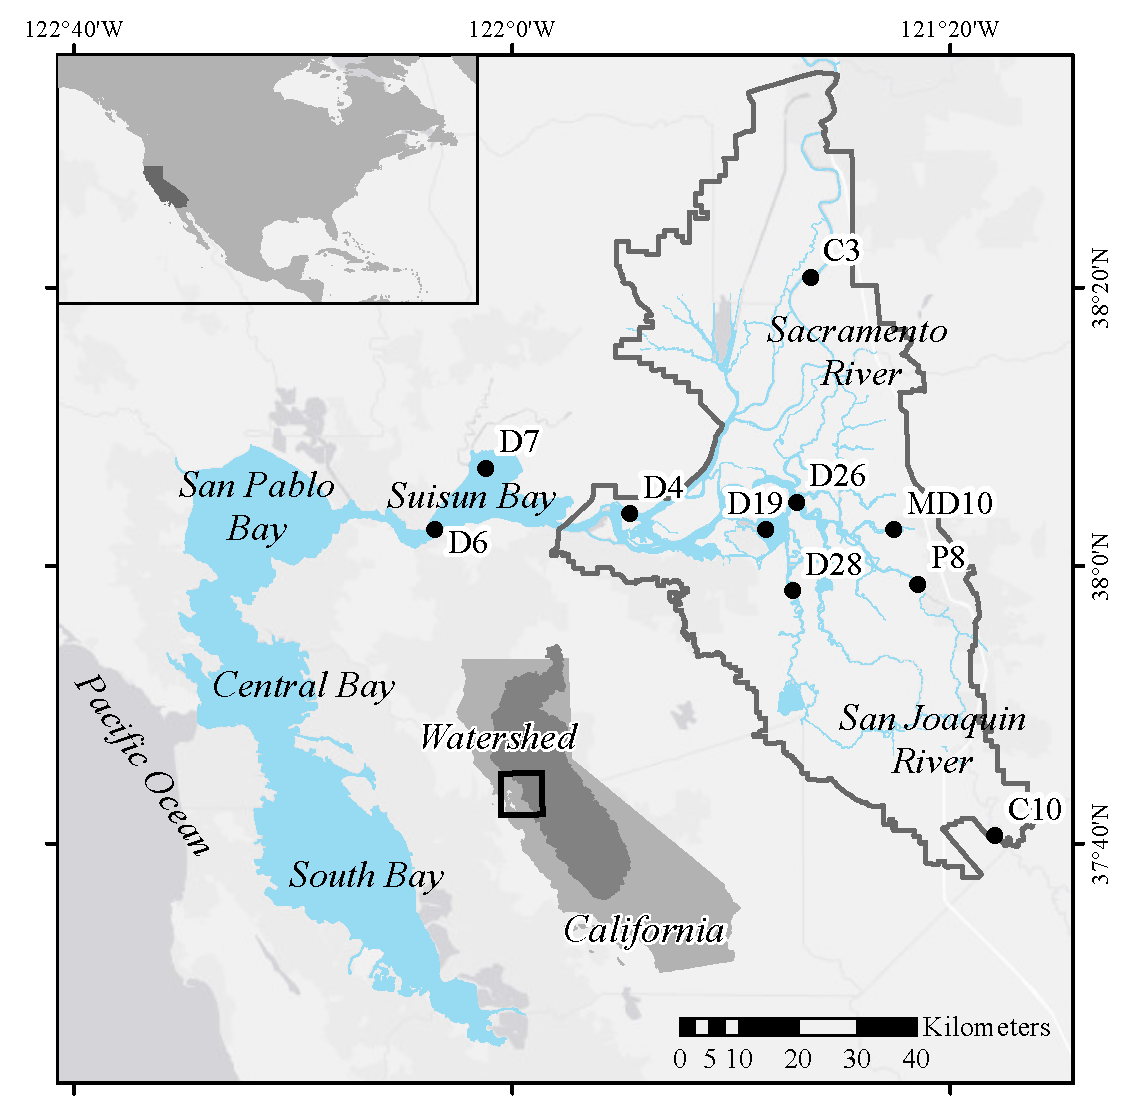
\includegraphics[width=0.8\textwidth,page=1]{figs/delt_map.pdf}
\caption{The \acl{sfe} Delta and monitoring stations used for analysis. The Delta drains the combined watershed from the Sacramento and San Joaquin rivers (bottom left). All data were obtained from the \acl{iep} website (\url{http://water.ca.gov/bdma/meta/Discrete/data.cfm})\cite{IEP13}.}
\label{fig:delt_map}   
\end{figure}

\begin{figure}[!ht]

{\centering 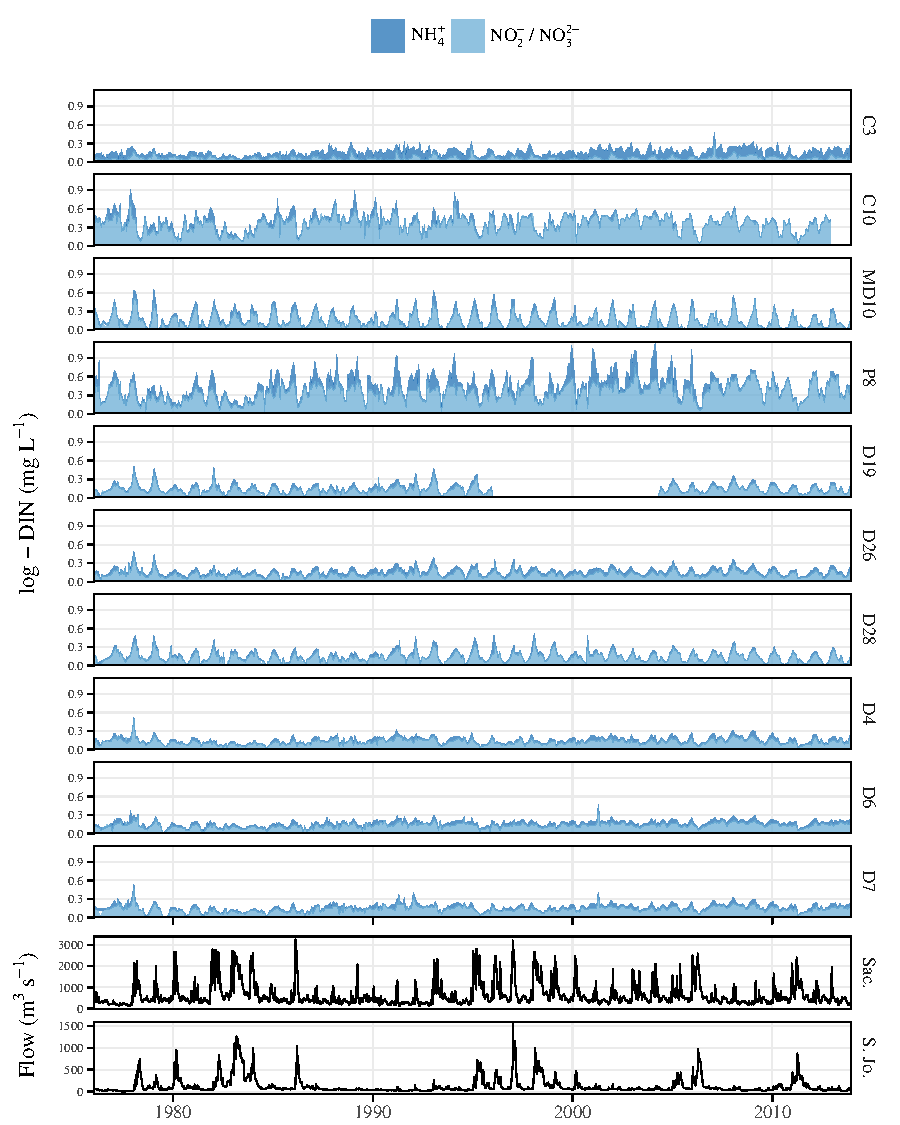
\includegraphics[width=0.9\textwidth]{figs/obsdat-1} 

}

\caption{Observed \ac{din} (NH$_4^{+}$ + NO$_2^{-}$/NO$_3^{2-}$) from ten stations in the upper \ac{sfe} Delta and flow from the Sacramento and San Joaquin rivers.  Data were collected monthly and evaluated with \ac{wrtds} models using daily flow estimates from 1976 to 2013. Note different y-axis scales.  See \cref{fig:delt_map} for station locations.}\label{fig:obsdat}
\end{figure}





\begin{figure}
\centering
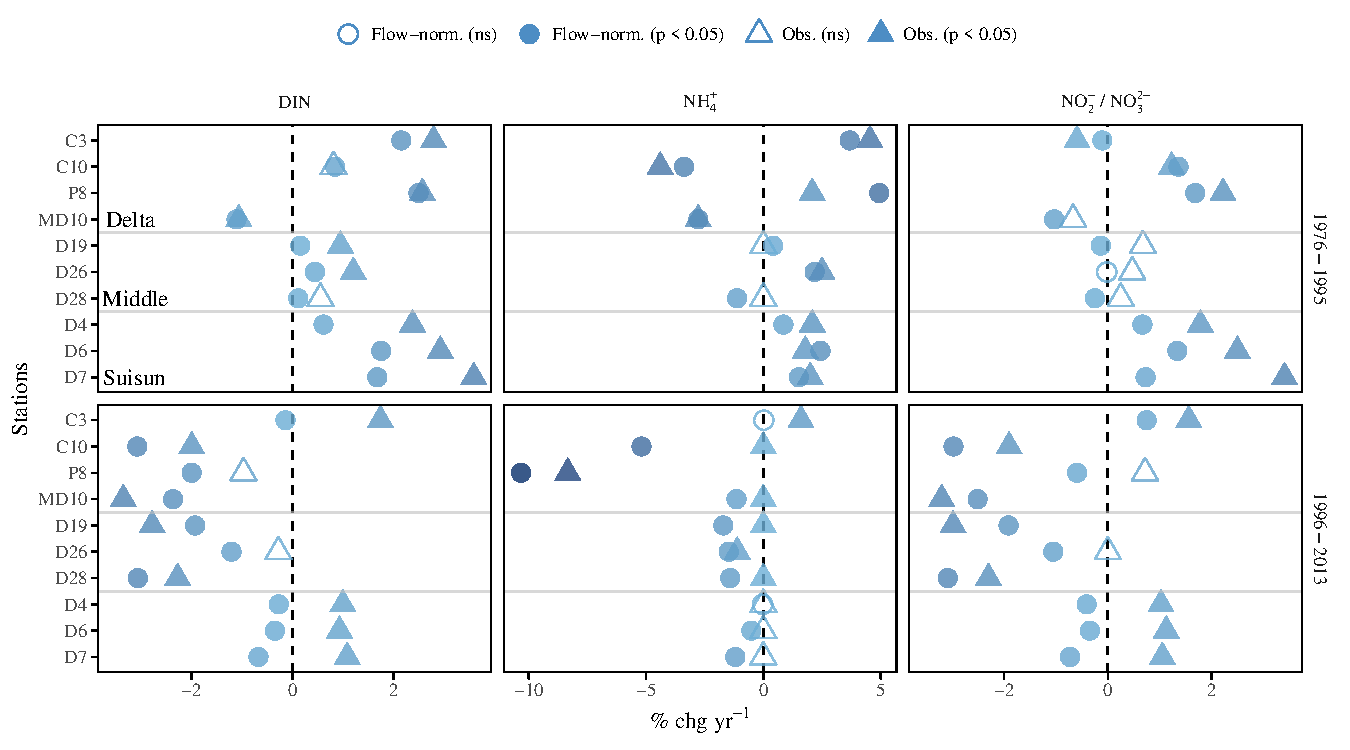
\includegraphics[width=1\textwidth,page=1]{figs/trndcomp1.pdf}
\caption{Results from seasonal Kendall tests on observed data (triangles) and flow-normalized predictions (circles) from \ac{wrtds} for nitrogen analytes. Results are shown as the percent change per year as the estimated Theil-Sen slope divided by the median for a given aggregation period (significance evaluated at $\alpha = 0.05$, based on $\tau$). Trends are shown separately for different annual groupings. See \cref{fig:trndcomp2,fig:trndcomp3} for seasonal groupings.}
\label{fig:trndcomp1}   
\end{figure}

\begin{figure}[!ht]

{\centering 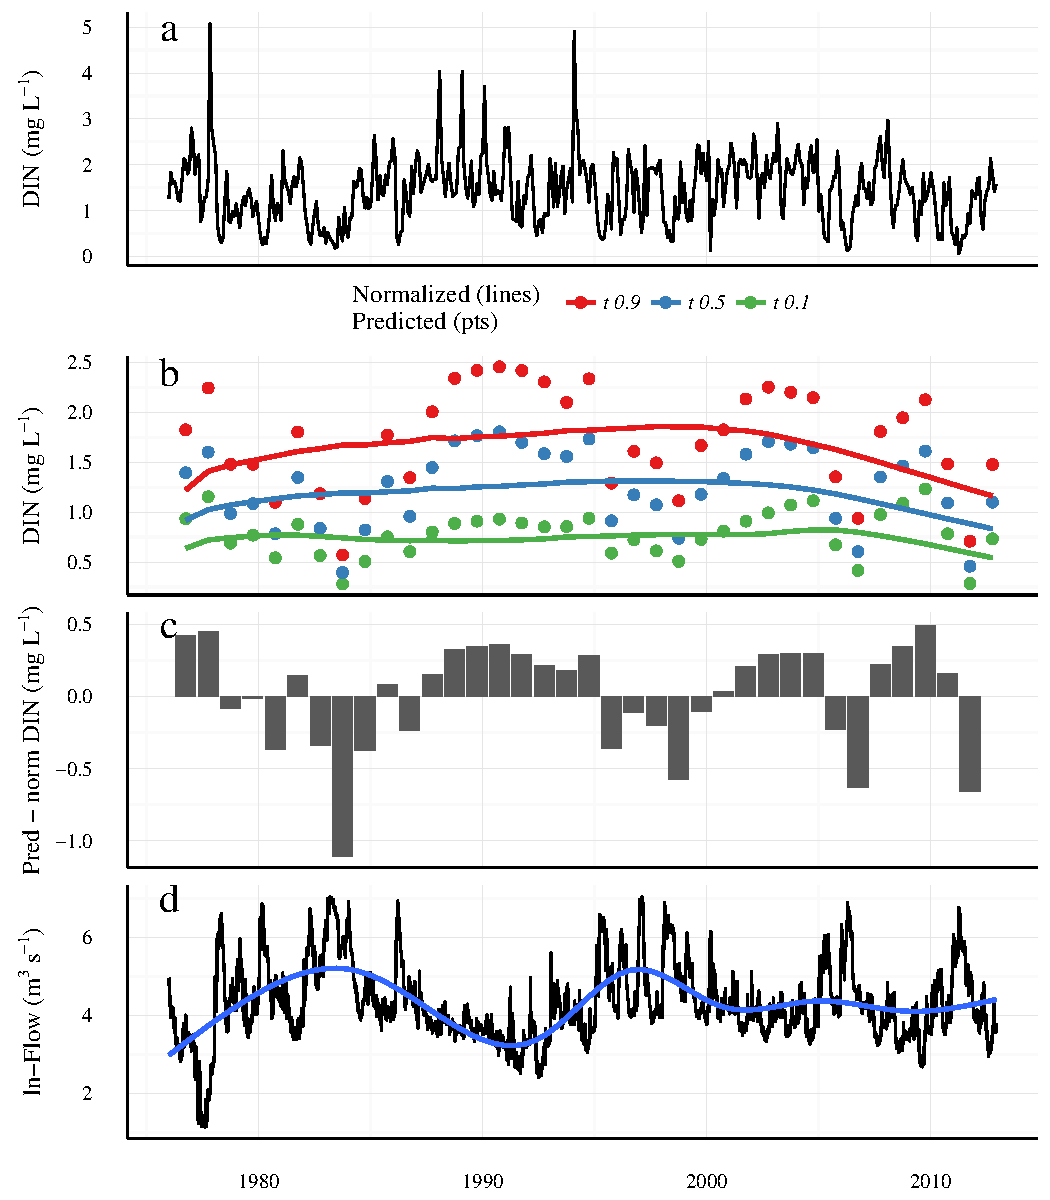
\includegraphics[width=0.75\textwidth]{figs/dinc10-1} 

}

\caption{Time series of \ac{din} and flow at station C10.  Subfigure (a) shows the observed \ac{din} time series and subfigure (b) shows the annual (water year starting in October) predictions from \ac{wrtds} for the conditional mean response.  The points in subfigure (b) are predictions of observed \ac{din} and the lines are flow-normalized predictions.  Subfigure (c) shows the difference between the model predictions and flow-normalized predictions.  Subfigure (d) shows the flow time series of the San Joaquin River with a locally-estimated (loess) smooth to emphasize the long-term trend. Subfigure (e) shows the modelled relationships between \ac{din}, flow, and time. Flow values in (e) are truncated by 5\textsuperscript{th} and 95\textsuperscript{th} percentiles of observed.}\label{fig:dinc10}
\end{figure}



\begin{figure}[!ht]

{\centering 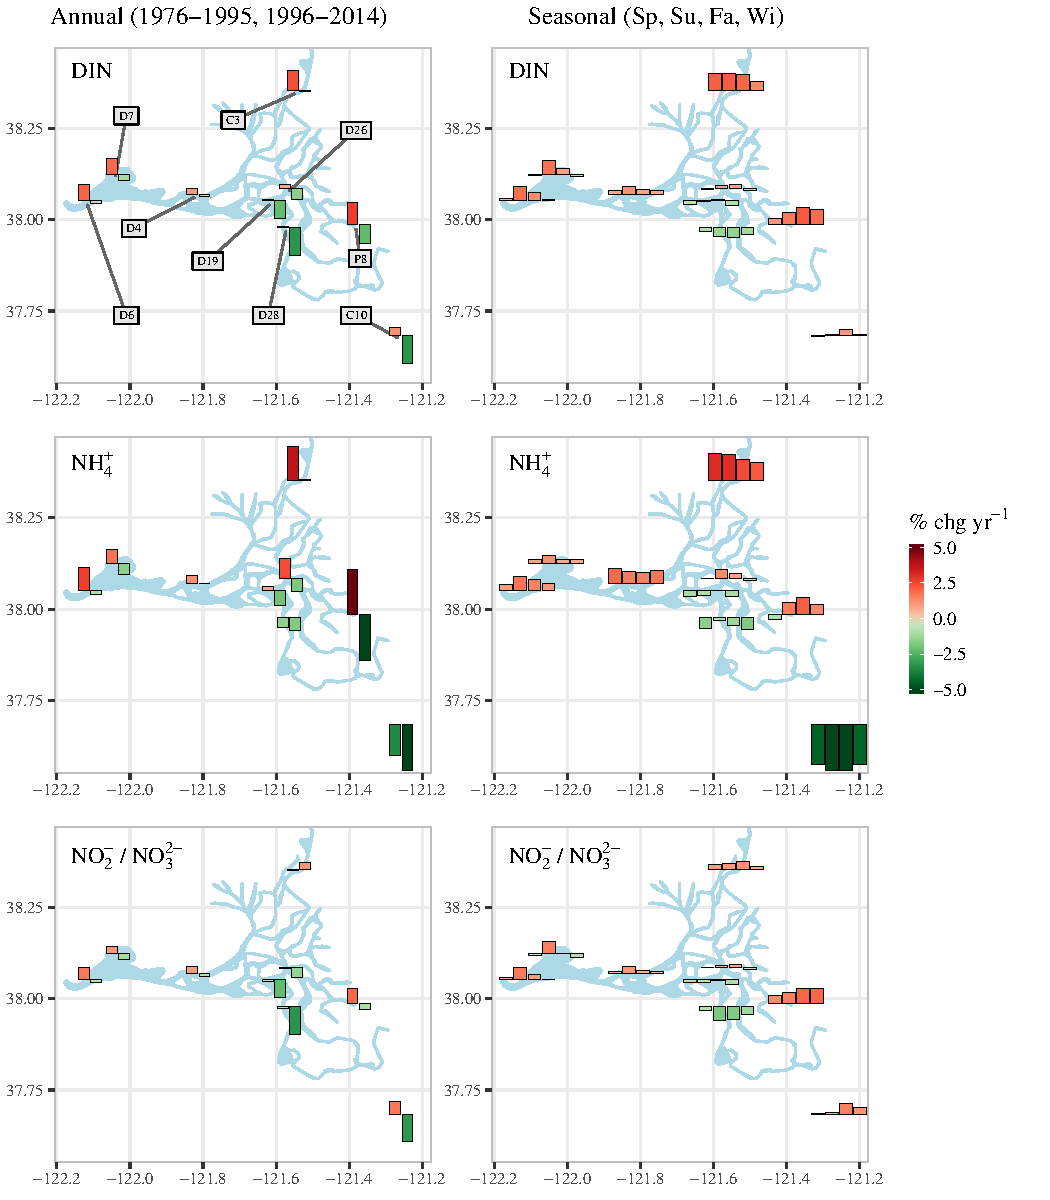
\includegraphics[width=0.7\textwidth]{figs/trndmap-1} 

}

\caption[Percent change per year in nitrogen analytes for aggregations by seasons from (a) 1976-1995 and (b) 1996-2013]{Percent change per year in nitrogen analytes for aggregations by seasons from (a) 1976-1995 and (b) 1996-2013.  Changes are based on seasonal Kendall tests of flow-normalized results within each time period. Station names are shown in the top left panel. Station locations have been jittered to reduce overlap. Months for each season are Spring: MAM, Summer: JJA, Fall: SON, Winter: DJF.}\label{fig:trndmap}
\end{figure}



\begin{figure}[!ht]

{\centering 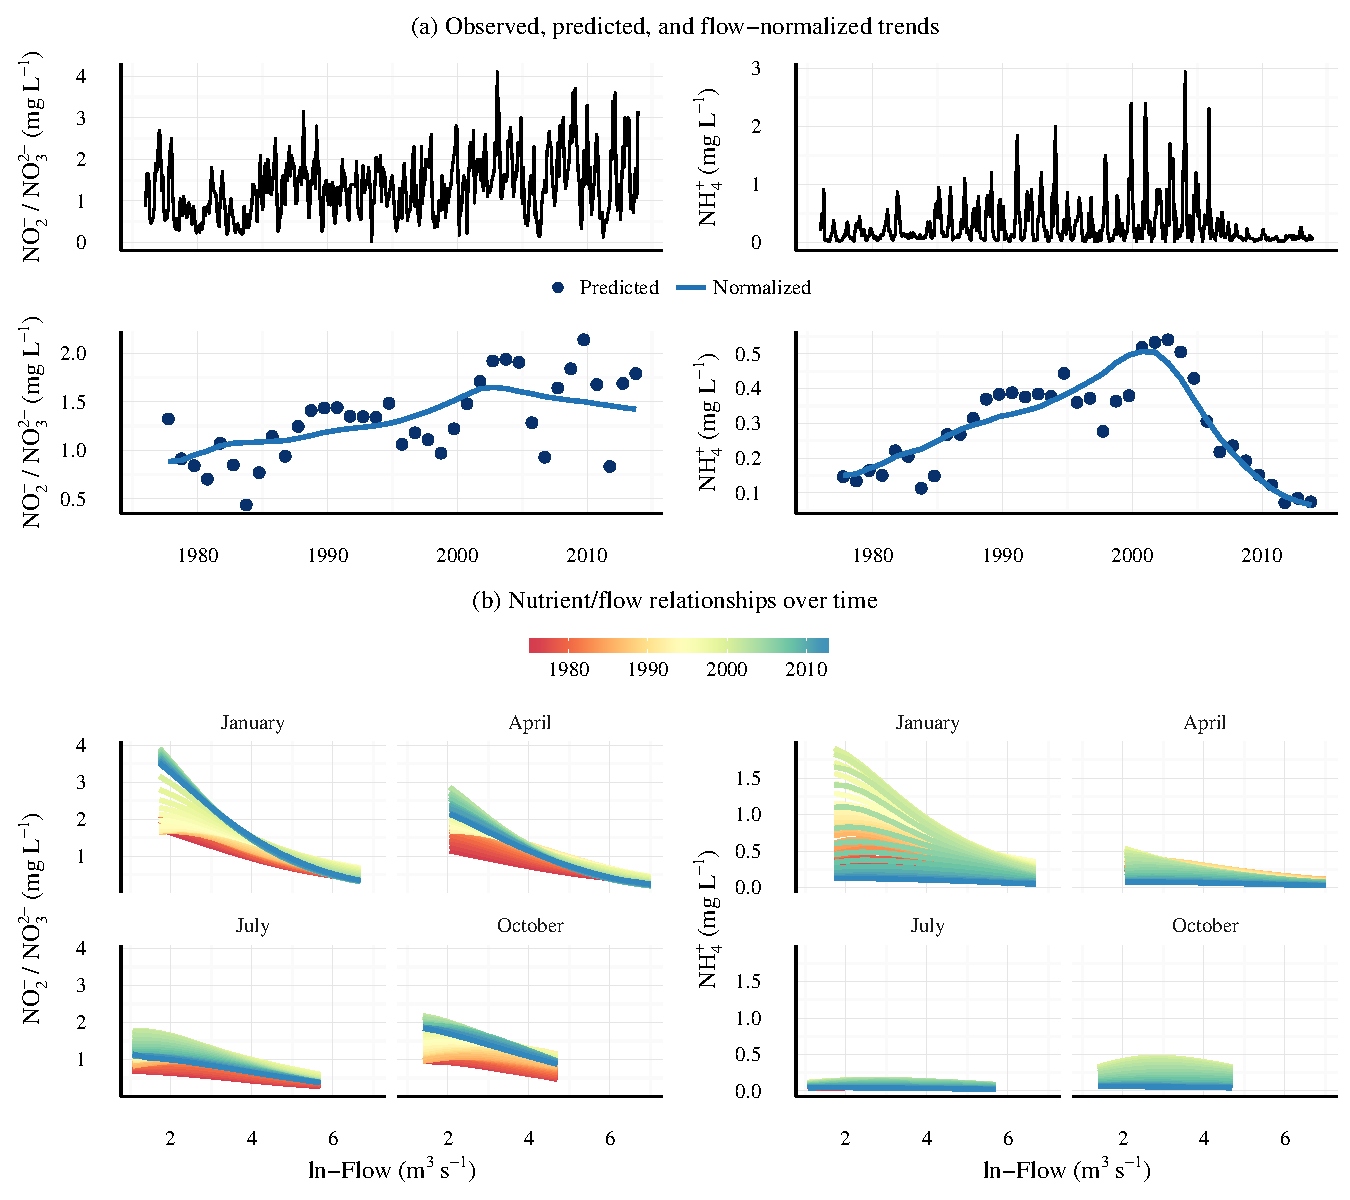
\includegraphics[width=\textwidth]{figs/p8trnds-1} 

}

\caption{Nitrogen trends at P8 as observed (a, top), predicted and flow-normalized estimates from \ac{wrtds} (a, bottom), and relationships with flow over time (b).  Nitrite/nitrate trends are on the left and ammonium trends are on the right.  Wastewater treatment plant upgrades at the City of Stockton (San Joaquin County) were completed in 2006 (\cref{fig:stock}), coincident with a dramatic decrease in ammonium at P8.}\label{fig:p8trnds}
\end{figure}



\begin{figure}[!ht]

{\centering 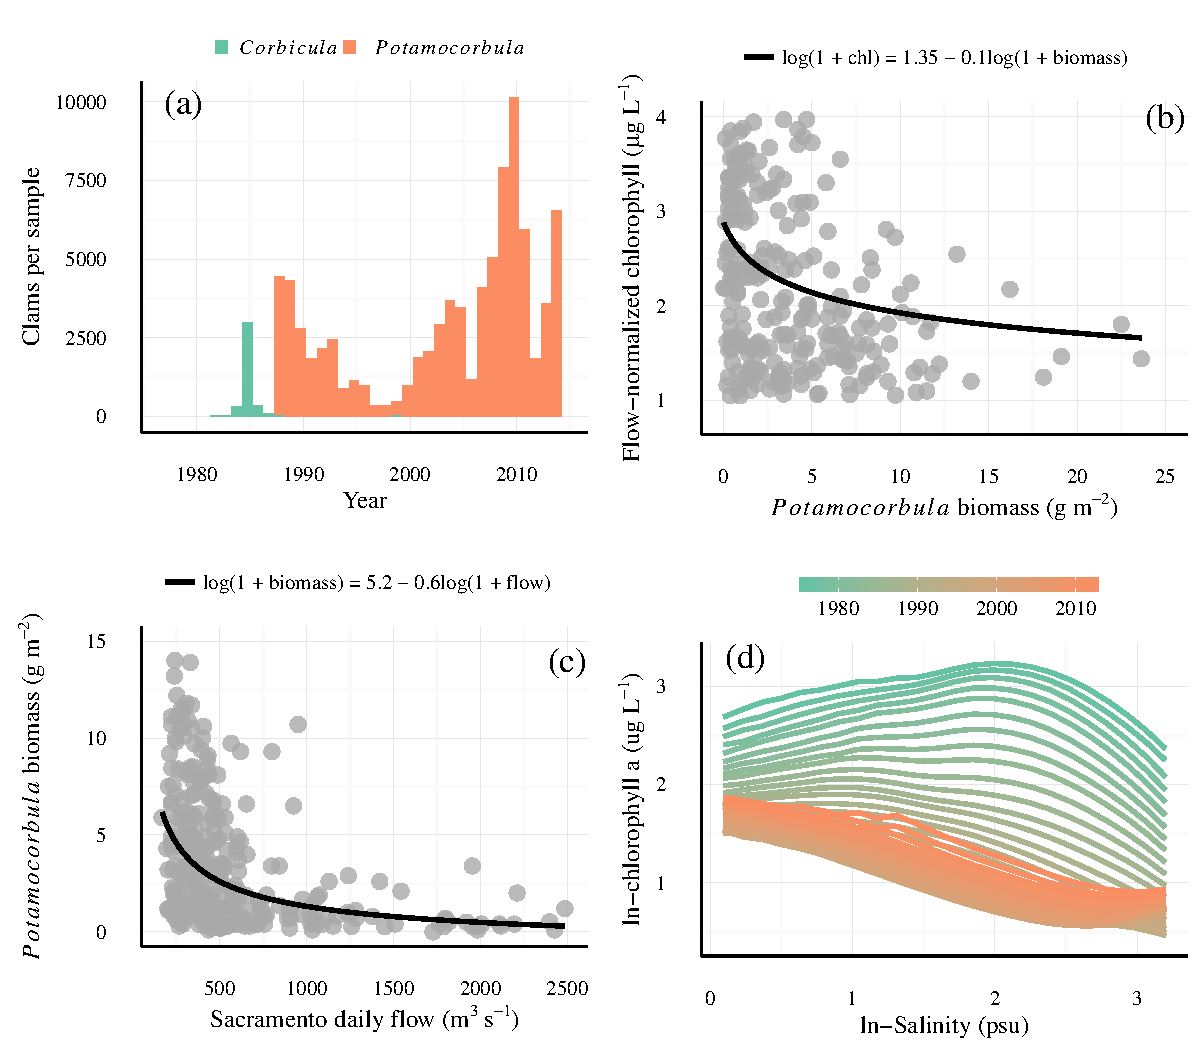
\includegraphics[width=0.9\textwidth]{figs/clmchl-1} 

}

\caption{Trends in clam abundance and \ac{chla} concentration from 1976 to 2013 at station D7 in Suisun Bay.  Invasion by \textit{Potamocorbula amurensis} clams in the late 1980s and displacement of \textit{Corbicula fluminea} was shown by changes in clam density (a, annual means),with biomass linked to salinity (b).  A coincident decrease in \ac{chla} concentration was also observed by changes in annual (c) and seasonal trends(d).  A significant ($p < 0.001$) relationship between clam biomass and \ac{chla} concentration is shown in subfigure (e).  Flow relationships with \ac{chla} concentration have also changed over time (f, observations from June).}\label{fig:clmchl}
\end{figure}



\clearpage
%%%%%%
% tables

% overall trends, years
%latex.default(tab[, -c(1, 2)], file = "", rowlabel = "Analyte/Station",     caption = cap.val, caption.loc = "top", rgroup = vars, n.rgroup = rep(nrow(tab)/3,         3), cgroup = c("Annual"), n.cgroup = c(2), rowname = stats,     label = "tab:trndsann", insert.bottom = foot.val)%
\begin{table}[!tbp]
\caption{Summaries of flow-normalized trends in nitrogen analytes for all stations and annual aggregations.  Summaries are  medians (mg L$^{-1}$) and percent change per year in parentheses (increasing in bold-italic). Changes and significance estimates are based on seasonal Kendall tests of flow-normalized results within each time period. See \cref{fig:trndmap} for a summary of spatial trends.\label{tab:trndsann}} 
\begin{center}
\begin{tabular}{lll}
\hline\hline
\multicolumn{1}{l}{\bfseries Analyte/Station}&\multicolumn{2}{c}{\bfseries Annual}\tabularnewline
\cline{2-3}
\multicolumn{1}{l}{}&\multicolumn{1}{c}{1976-1995}&\multicolumn{1}{c}{1996-2013}\tabularnewline
\hline
{\bfseries DIN}&&\tabularnewline
~~C10&1.3 \footnotesize{(\textit{\textbf{0.8}})**}&1.4 \footnotesize{(-3.1)**}\tabularnewline
~~C3&0.3 \footnotesize{(\textit{\textbf{2.2}})**}&0.5 \footnotesize{(-0.1)**}\tabularnewline
~~D19&0.4 \footnotesize{(\textit{\textbf{0.2}})**}&0.4 \footnotesize{(-1.9)**}\tabularnewline
~~D26&0.4 \footnotesize{(\textit{\textbf{0.4}})**}&0.5 \footnotesize{(-1.2)**}\tabularnewline
~~D28&0.4 \footnotesize{(\textit{\textbf{0.1}})**}&0.4 \footnotesize{(-3.1)**}\tabularnewline
~~D4&0.3 \footnotesize{(\textit{\textbf{0.6}})**}&0.4 \footnotesize{(-0.3)**}\tabularnewline
~~D6&0.4 \footnotesize{(\textit{\textbf{1.8}})**}&0.5 \footnotesize{(-0.3)**}\tabularnewline
~~D7&0.4 \footnotesize{(\textit{\textbf{1.7}})**}&0.5 \footnotesize{(-0.7)**}\tabularnewline
~~MD10&0.4 \footnotesize{(-1.1)**}&0.3 \footnotesize{(-2.4)**}\tabularnewline
~~P8&1.3 \footnotesize{(\textit{\textbf{2.5}})**}&1.7 \footnotesize{(-2)**}\tabularnewline
\hline
{\bfseries NH$_{4}^{+}$}&&\tabularnewline
~~C10&0.1 \footnotesize{(-3.4)**}&0 \footnotesize{(-5.2)**}\tabularnewline
~~C3&0.2 \footnotesize{(\textit{\textbf{3.7}})**}&0.3 \footnotesize{(\textit{\textbf{0}})}\tabularnewline
~~D19&0 \footnotesize{(\textit{\textbf{0.4}})**}&0 \footnotesize{(-1.7)**}\tabularnewline
~~D26&0.1 \footnotesize{(\textit{\textbf{2.2}})**}&0.1 \footnotesize{(-1.5)**}\tabularnewline
~~D28&0 \footnotesize{(-1.1)**}&0 \footnotesize{(-1.4)**}\tabularnewline
~~D4&0 \footnotesize{(\textit{\textbf{0.9}})**}&0.1 \footnotesize{(\textit{\textbf{0}})}\tabularnewline
~~D6&0.1 \footnotesize{(\textit{\textbf{2.4}})**}&0.1 \footnotesize{(-0.5)**}\tabularnewline
~~D7&0.1 \footnotesize{(\textit{\textbf{1.5}})**}&0.1 \footnotesize{(-1.2)**}\tabularnewline
~~MD10&0.1 \footnotesize{(-2.8)**}&0 \footnotesize{(-1.1)**}\tabularnewline
~~P8&0.2 \footnotesize{(\textit{\textbf{4.9}})**}&0.1 \footnotesize{(-10.3)**}\tabularnewline
\hline
{\bfseries NO$_{2}^{-}$/NO$_{3}^{2-}$}&&\tabularnewline
~~C10&1.2 \footnotesize{(\textit{\textbf{1.4}})**}&1.4 \footnotesize{(-3)**}\tabularnewline
~~C3&0.1 \footnotesize{(-0.1)**}&0.2 \footnotesize{(\textit{\textbf{0.7}})**}\tabularnewline
~~D19&0.4 \footnotesize{(-0.1)**}&0.4 \footnotesize{(-1.9)**}\tabularnewline
~~D26&0.3 \footnotesize{(\textit{\textbf{0}})}&0.4 \footnotesize{(-1.1)**}\tabularnewline
~~D28&0.4 \footnotesize{(-0.2)**}&0.4 \footnotesize{(-3.1)**}\tabularnewline
~~D4&0.3 \footnotesize{(\textit{\textbf{0.7}})**}&0.3 \footnotesize{(-0.4)**}\tabularnewline
~~D6&0.3 \footnotesize{(\textit{\textbf{1.3}})**}&0.4 \footnotesize{(-0.3)**}\tabularnewline
~~D7&0.4 \footnotesize{(\textit{\textbf{0.7}})**}&0.4 \footnotesize{(-0.7)**}\tabularnewline
~~MD10&0.4 \footnotesize{(-1)**}&0.3 \footnotesize{(-2.5)**}\tabularnewline
~~P8&1.2 \footnotesize{(\textit{\textbf{1.7}})**}&1.5 \footnotesize{(-0.6)**}\tabularnewline
\hline
\end{tabular}\end{center}

\footnotesize *$p<0.05$; **$p<0.005$\end{table}


% overall trends, seasons, first annual periodyears
%latex.default(tab[, -c(1, 2)], file = "", rowlabel = "Analyte/Station",     caption = cap.val, caption.loc = "top", rgroup = vars, n.rgroup = rep(nrow(tab)/3,         3), cgroup = c("Seasonal, 1976-1995"), n.cgroup = c(4),     rowname = stats, label = "tab:trndsbef", insert.bottom = foot.val)%
\begin{table}[!tbp]
\caption{Summaries of flow-normalized trends in nitrogen analytes for all stations and seasonal aggregations from 1976-1995. Summaries are  medians (mg L$^{-1}$) and percent change per year in parentheses (increasing in bold-italic). Changes and significance estimates are based on seasonal Kendall tests of flow-normalized results within each time period. See \cref{fig:trndmap} for a summary of spatial trends. Months for each season are Spring: MAM, Summer: JJA, Fall: SON, Winter: DJF.\label{tab:trndsbef}} 
\begin{center}
\begin{tabular}{lllll}
\hline\hline
\multicolumn{1}{l}{\bfseries Analyte/Station}&\multicolumn{4}{c}{\bfseries Seasonal, 1976-1995}\tabularnewline
\cline{2-5}
\multicolumn{1}{l}{}&\multicolumn{1}{c}{Spring}&\multicolumn{1}{c}{Summer}&\multicolumn{1}{c}{Fall}&\multicolumn{1}{c}{Winter}\tabularnewline
\hline
{\bfseries DIN}&&&&\tabularnewline
~~C10&1.2 \footnotesize{(\textit{\textbf{1.1}})**}&1.2 \footnotesize{(\textit{\textbf{0.3}})}&1.3 \footnotesize{(\textit{\textbf{0.5}})**}&1.7 \footnotesize{(\textit{\textbf{1.2}})**}\tabularnewline
~~C3&0.3 \footnotesize{(\textit{\textbf{2.4}})**}&0.3 \footnotesize{(\textit{\textbf{2.3}})**}&0.4 \footnotesize{(\textit{\textbf{2.4}})**}&0.4 \footnotesize{(\textit{\textbf{1.9}})**}\tabularnewline
~~D19&0.5 \footnotesize{(\textit{\textbf{0.3}})}&0.2 \footnotesize{(\textit{\textbf{0.4}})}&0.3 \footnotesize{(\textit{\textbf{0.7}})**}&0.7 \footnotesize{(-0.2)}\tabularnewline
~~D26&0.4 \footnotesize{(\textit{\textbf{0.7}})**}&0.3 \footnotesize{(\textit{\textbf{0.4}})*}&0.4 \footnotesize{(\textit{\textbf{1}})**}&0.6 \footnotesize{(\textit{\textbf{0.3}})}\tabularnewline
~~D28&0.5 \footnotesize{(\textit{\textbf{0.8}})*}&0.2 \footnotesize{(\textit{\textbf{0.3}})}&0.3 \footnotesize{(\textit{\textbf{0.5}})*}&0.8 \footnotesize{(-0.3)}\tabularnewline
~~D4&0.4 \footnotesize{(\textit{\textbf{0.2}})}&0.3 \footnotesize{(\textit{\textbf{1.4}})**}&0.3 \footnotesize{(\textit{\textbf{1.1}})**}&0.5 \footnotesize{(-0.5)}\tabularnewline
~~D6&0.4 \footnotesize{(\textit{\textbf{0.4}})}&0.3 \footnotesize{(\textit{\textbf{4.6}})**}&0.4 \footnotesize{(\textit{\textbf{1.4}})**}&0.5 \footnotesize{(-0.7)*}\tabularnewline
~~D7&0.4 \footnotesize{(-0.2)}&0.3 \footnotesize{(\textit{\textbf{4.2}})**}&0.4 \footnotesize{(\textit{\textbf{1.5}})**}&0.6 \footnotesize{(-2.4)**}\tabularnewline
~~MD10&0.6 \footnotesize{(-0.3)}&0.2 \footnotesize{(-3.6)**}&0.3 \footnotesize{(\textit{\textbf{0.8}})**}&1.3 \footnotesize{(-0.3)*}\tabularnewline
~~P8&1.3 \footnotesize{(\textit{\textbf{2.4}})**}&0.9 \footnotesize{(\textit{\textbf{2.4}})**}&1.3 \footnotesize{(\textit{\textbf{3.1}})**}&1.9 \footnotesize{(\textit{\textbf{2.1}})**}\tabularnewline
\hline
{\bfseries NH$_{4}^{+}$}&&&&\tabularnewline
~~C10&0.1 \footnotesize{(-2.3)**}&0 \footnotesize{(-6.8)**}&0.1 \footnotesize{(-7.1)**}&0.3 \footnotesize{(-1.5)**}\tabularnewline
~~C3&0.2 \footnotesize{(\textit{\textbf{3.9}})**}&0.2 \footnotesize{(\textit{\textbf{4}})**}&0.3 \footnotesize{(\textit{\textbf{3.8}})**}&0.2 \footnotesize{(\textit{\textbf{2.9}})**}\tabularnewline
~~D19&0.1 \footnotesize{(\textit{\textbf{0.4}})*}&0 \footnotesize{(-1.7)**}&0 \footnotesize{(\textit{\textbf{1.2}})**}&0.1 \footnotesize{(\textit{\textbf{2.5}})**}\tabularnewline
~~D26&0.1 \footnotesize{(\textit{\textbf{1.4}})**}&0.1 \footnotesize{(\textit{\textbf{2.5}})**}&0.1 \footnotesize{(\textit{\textbf{3.1}})**}&0.1 \footnotesize{(\textit{\textbf{2.3}})**}\tabularnewline
~~D28&0.1 \footnotesize{(-0.5)}&0 \footnotesize{(-3.7)**}&0 \footnotesize{(-1.6)**}&0.1 \footnotesize{(\textit{\textbf{1.7}})**}\tabularnewline
~~D4&0.1 \footnotesize{(\textit{\textbf{1.7}})**}&0 \footnotesize{(\textit{\textbf{1}})**}&0 \footnotesize{(-0.7)}&0.1 \footnotesize{(\textit{\textbf{2}})**}\tabularnewline
~~D6&0.1 \footnotesize{(\textit{\textbf{2.9}})**}&0.1 \footnotesize{(\textit{\textbf{2.8}})**}&0.1 \footnotesize{(-0.1)}&0.1 \footnotesize{(\textit{\textbf{2.1}})**}\tabularnewline
~~D7&0.1 \footnotesize{(\textit{\textbf{3.3}})**}&0 \footnotesize{(\textit{\textbf{2}})**}&0.1 \footnotesize{(-2.8)**}&0.1 \footnotesize{(\textit{\textbf{1.7}})**}\tabularnewline
~~MD10&0.1 \footnotesize{(-1.8)**}&0 \footnotesize{(-6.5)**}&0 \footnotesize{(-3.3)**}&0.2 \footnotesize{(\textit{\textbf{0.4}})}\tabularnewline
~~P8&0.2 \footnotesize{(\textit{\textbf{3.9}})**}&0.1 \footnotesize{(\textit{\textbf{1.8}})**}&0.2 \footnotesize{(\textit{\textbf{7}})**}&0.6 \footnotesize{(\textit{\textbf{7}})**}\tabularnewline
\hline
{\bfseries NO$_{2}^{-}$/NO$_{3}^{2-}$}&&&&\tabularnewline
~~C10&1.1 \footnotesize{(\textit{\textbf{1.5}})**}&1.2 \footnotesize{(\textit{\textbf{0.6}})**}&1.2 \footnotesize{(\textit{\textbf{1.3}})**}&1.5 \footnotesize{(\textit{\textbf{1.8}})**}\tabularnewline
~~C3&0.2 \footnotesize{(\textit{\textbf{0.7}})**}&0.1 \footnotesize{(-1)**}&0.1 \footnotesize{(-0.3)}&0.2 \footnotesize{(\textit{\textbf{1}})**}\tabularnewline
~~D19&0.4 \footnotesize{(\textit{\textbf{0.4}})}&0.2 \footnotesize{(-0.3)}&0.3 \footnotesize{(\textit{\textbf{0.3}})}&0.6 \footnotesize{(-0.9)*}\tabularnewline
~~D26&0.4 \footnotesize{(\textit{\textbf{0.6}})*}&0.2 \footnotesize{(-0.1)}&0.3 \footnotesize{(\textit{\textbf{0.3}})*}&0.5 \footnotesize{(-0.3)}\tabularnewline
~~D28&0.5 \footnotesize{(\textit{\textbf{0.7}})*}&0.2 \footnotesize{(-0.1)}&0.3 \footnotesize{(\textit{\textbf{0.2}})}&0.7 \footnotesize{(-1)**}\tabularnewline
~~D4&0.3 \footnotesize{(\textit{\textbf{0.1}})}&0.3 \footnotesize{(\textit{\textbf{1.4}})**}&0.3 \footnotesize{(\textit{\textbf{1.1}})**}&0.4 \footnotesize{(-0.8)*}\tabularnewline
~~D6&0.4 \footnotesize{(-0.2)}&0.3 \footnotesize{(\textit{\textbf{4.1}})**}&0.3 \footnotesize{(\textit{\textbf{1.4}})**}&0.4 \footnotesize{(-1)**}\tabularnewline
~~D7&0.4 \footnotesize{(-1)*}&0.3 \footnotesize{(\textit{\textbf{3.4}})**}&0.4 \footnotesize{(\textit{\textbf{0.4}})}&0.4 \footnotesize{(-3.6)**}\tabularnewline
~~MD10&0.5 \footnotesize{(-0.2)}&0.2 \footnotesize{(-3.6)**}&0.2 \footnotesize{(\textit{\textbf{1.5}})**}&1.2 \footnotesize{(-0.5)*}\tabularnewline
~~P8&1.2 \footnotesize{(\textit{\textbf{2}})**}&0.9 \footnotesize{(\textit{\textbf{2.3}})**}&1.1 \footnotesize{(\textit{\textbf{2}})**}&1.4 \footnotesize{(\textit{\textbf{1}})**}\tabularnewline
\hline
\end{tabular}\end{center}

\footnotesize *$p<0.05$; **$p<0.005$\end{table}


% overall trends, seasons, first annual periodyears
%latex.default(tab[, -c(1, 2)], file = "", rowlabel = "Analyte/Station",     caption = cap.val, caption.loc = "top", rgroup = vars, n.rgroup = rep(nrow(tab)/3,         3), cgroup = c("Seasonal, 1996-2013"), n.cgroup = c(4),     rowname = stats, label = "tab:trndsaft", insert.bottom = foot.val)%
\begin{table}[!tbp]
\caption{Summaries of flow-normalized trends in nitrogen analytes for all stations and seasonal aggregations from 1996-2013. Summaries are  medians (mg L$^{-1}$) and percent change per year in parentheses (increasing in bold-italic). Changes and significance estimates are based on seasonal Kendall tests of flow-normalized results within each time period. See \cref{fig:trndmap} for a summary of spatial trends. Months for each season are Spring: MAM, Summer: JJA, Fall: SON, Winter: DJF.\label{tab:trndsaft}} 
\begin{center}
\begin{tabular}{lllll}
\hline\hline
\multicolumn{1}{l}{\bfseries Analyte/Station}&\multicolumn{4}{c}{\bfseries Seasonal, 1996-2013}\tabularnewline
\cline{2-5}
\multicolumn{1}{l}{}&\multicolumn{1}{c}{Spring}&\multicolumn{1}{c}{Summer}&\multicolumn{1}{c}{Fall}&\multicolumn{1}{c}{Winter}\tabularnewline
\hline
{\bfseries DIN}&&&&\tabularnewline
~~C10&1.1 \footnotesize{(-4.1)**}&1.3 \footnotesize{(-3.1)**}&1.6 \footnotesize{(-2)**}&1.7 \footnotesize{(-3.4)**}\tabularnewline
~~C3&0.5 \footnotesize{(\textit{\textbf{0.5}})}&0.4 \footnotesize{(\textit{\textbf{0.1}})}&0.6 \footnotesize{(-0.2)}&0.5 \footnotesize{(-0.6)**}\tabularnewline
~~D19&0.5 \footnotesize{(-2.8)**}&0.2 \footnotesize{(-1)*}&0.3 \footnotesize{(-1.6)**}&0.7 \footnotesize{(-2.3)**}\tabularnewline
~~D26&0.5 \footnotesize{(-1.9)**}&0.3 \footnotesize{(-1.7)**}&0.4 \footnotesize{(-1)**}&0.6 \footnotesize{(-0.8)**}\tabularnewline
~~D28&0.5 \footnotesize{(-3)**}&0.2 \footnotesize{(-4.9)**}&0.2 \footnotesize{(-4.9)**}&0.7 \footnotesize{(-2.1)**}\tabularnewline
~~D4&0.4 \footnotesize{(\textit{\textbf{0}})}&0.4 \footnotesize{(-1)**}&0.4 \footnotesize{(-0.9)**}&0.5 \footnotesize{(\textit{\textbf{0.6}})**}\tabularnewline
~~D6&0.5 \footnotesize{(-0.2)*}&0.5 \footnotesize{(-1)**}&0.5 \footnotesize{(-0.3)*}&0.5 \footnotesize{(-0.1)}\tabularnewline
~~D7&0.5 \footnotesize{(-0.8)**}&0.4 \footnotesize{(-1.3)**}&0.4 \footnotesize{(-0.4)**}&0.6 \footnotesize{(-0.2)}\tabularnewline
~~MD10&0.4 \footnotesize{(-2.3)**}&0.2 \footnotesize{(-3.7)**}&0.2 \footnotesize{(-4.4)**}&1 \footnotesize{(-1.8)**}\tabularnewline
~~P8&1.5 \footnotesize{(-1.9)**}&1.2 \footnotesize{(-3.5)**}&1.8 \footnotesize{(-2.4)**}&2.7 \footnotesize{(-2.2)**}\tabularnewline
\hline
{\bfseries NH$_{4}^{+}$}&&&&\tabularnewline
~~C10&0 \footnotesize{(-4.2)**}&0 \footnotesize{(-6.1)**}&0 \footnotesize{(-8.5)**}&0.1 \footnotesize{(-7.3)**}\tabularnewline
~~C3&0.3 \footnotesize{(\textit{\textbf{1}})**}&0.3 \footnotesize{(-0.8)*}&0.4 \footnotesize{(-0.5)*}&0.2 \footnotesize{(-0.1)}\tabularnewline
~~D19&0 \footnotesize{(-1.9)**}&0 \footnotesize{(-0.4)}&0 \footnotesize{(-2.2)**}&0.1 \footnotesize{(-1.8)**}\tabularnewline
~~D26&0.1 \footnotesize{(-1.2)**}&0.1 \footnotesize{(-1.3)**}&0.1 \footnotesize{(-1.9)**}&0.1 \footnotesize{(-1.4)**}\tabularnewline
~~D28&0 \footnotesize{(-1.7)**}&0 \footnotesize{(-0.2)}&0 \footnotesize{(-2.4)**}&0.1 \footnotesize{(-3.1)**}\tabularnewline
~~D4&0.1 \footnotesize{(\textit{\textbf{0.3}})}&0 \footnotesize{(-1.3)**}&0.1 \footnotesize{(-0.3)}&0.1 \footnotesize{(\textit{\textbf{1}})**}\tabularnewline
~~D6&0.1 \footnotesize{(-0.7)**}&0.1 \footnotesize{(-1)**}&0.1 \footnotesize{(\textit{\textbf{0.3}})}&0.1 \footnotesize{(-0.3)**}\tabularnewline
~~D7&0.1 \footnotesize{(-2.2)**}&0 \footnotesize{(-2.1)**}&0.1 \footnotesize{(\textit{\textbf{1.3}})**}&0.1 \footnotesize{(-0.4)*}\tabularnewline
~~MD10&0 \footnotesize{(-1.4)*}&0 \footnotesize{(-0.1)}&0 \footnotesize{(-0.8)**}&0.1 \footnotesize{(-4.3)**}\tabularnewline
~~P8&0.2 \footnotesize{(-8.7)**}&0.1 \footnotesize{(-6.3)**}&0.2 \footnotesize{(-10.4)**}&0.5 \footnotesize{(-13.1)**}\tabularnewline
\hline
{\bfseries NO$_{2}^{-}$/NO$_{3}^{2-}$}&&&&\tabularnewline
~~C10&1.1 \footnotesize{(-4.2)**}&1.2 \footnotesize{(-3.2)**}&1.6 \footnotesize{(-1.9)**}&1.6 \footnotesize{(-3.3)**}\tabularnewline
~~C3&0.2 \footnotesize{(\textit{\textbf{0.4}})}&0.1 \footnotesize{(\textit{\textbf{3.1}})**}&0.2 \footnotesize{(\textit{\textbf{1.7}})**}&0.2 \footnotesize{(-0.4)}\tabularnewline
~~D19&0.4 \footnotesize{(-2.9)**}&0.2 \footnotesize{(-1)*}&0.3 \footnotesize{(-1.5)**}&0.6 \footnotesize{(-2.2)**}\tabularnewline
~~D26&0.4 \footnotesize{(-1.9)**}&0.2 \footnotesize{(-1.6)**}&0.3 \footnotesize{(-0.6)*}&0.5 \footnotesize{(-0.6)**}\tabularnewline
~~D28&0.5 \footnotesize{(-3)**}&0.2 \footnotesize{(-5.4)**}&0.2 \footnotesize{(-5.2)**}&0.7 \footnotesize{(-1.7)**}\tabularnewline
~~D4&0.3 \footnotesize{(-0.1)}&0.3 \footnotesize{(-1)**}&0.3 \footnotesize{(-1)**}&0.4 \footnotesize{(\textit{\textbf{0.4}})**}\tabularnewline
~~D6&0.4 \footnotesize{(-0.1)}&0.4 \footnotesize{(-1)**}&0.4 \footnotesize{(-0.4)*}&0.4 \footnotesize{(-0.1)}\tabularnewline
~~D7&0.4 \footnotesize{(-0.6)**}&0.4 \footnotesize{(-1.2)**}&0.4 \footnotesize{(-0.8)**}&0.4 \footnotesize{(-0.3)*}\tabularnewline
~~MD10&0.4 \footnotesize{(-2.6)**}&0.1 \footnotesize{(-4.5)**}&0.2 \footnotesize{(-5.4)**}&1 \footnotesize{(-1.4)**}\tabularnewline
~~P8&1.3 \footnotesize{(-1.1)**}&1.1 \footnotesize{(-3.1)**}&1.6 \footnotesize{(-0.3)*}&2.2 \footnotesize{(\textit{\textbf{0}})}\tabularnewline
\hline
\end{tabular}\end{center}

\footnotesize *$p<0.05$; **$p<0.005$\end{table}


% trends in no23, nh at p8
%latex.default(totab, file = "", rowlabel = "Period", caption = cap.val,     caption.loc = "top", rgroup = segs, n.rgroup = c(2, rep(4,         2)), cgroup = vars, n.cgroup = c(2, 2), rowname = cats,     label = "tab:p8chg", insert.bottom = foot.val)%
\begin{table}[!tbp]
\caption{Summaries of flow-normalized trends in nitrite/nitrate and ammonium (mg L$^{-1}$) concentrations before and after \ac{wwtp} upgrades upstream of station P8. Upgrades were completed in 2006 at the City of Stockton \ac{wwtp} (San Joaquin County, \cref{fig:stock}).  Summaries are  medians and percent change per year in parentheses (increasing in bold-italic).  Changes and significance estimates are based on seasonal Kendall tests of flow-normalized results within each time period. Increasing values are in bold-italics. Months for each season are Spring: MAM, Summer: JJA, Fall: SON, Winter: DJF.\label{tab:p8chg}} 
\begin{center}
\begin{tabular}{lllcll}
\hline\hline
\multicolumn{1}{l}{\bfseries Period}&\multicolumn{2}{c}{\bfseries NO$_{2}^{-}$/NO$_{3}^{2-}$}&\multicolumn{1}{c}{\bfseries }&\multicolumn{2}{c}{\bfseries NH$_{4}^{+}$}\tabularnewline
\cline{2-3} \cline{5-6}
\multicolumn{1}{l}{}&\multicolumn{1}{c}{Median}&\multicolumn{1}{c}{\% change}&\multicolumn{1}{c}{}&\multicolumn{1}{c}{Median}&\multicolumn{1}{c}{\% change}\tabularnewline
\hline
{\bfseries Annual}&&&&&\tabularnewline
~~1976-2006&1.3&\textit{\textbf{2}}**&&0.2&\textit{\textbf{2.8}}**\tabularnewline
~~2007-2013&1.4&-1.9**&&0.1&-16.6**\tabularnewline
\hline
{\bfseries Seasonal, pre}&&&&&\tabularnewline
~~Spring&1.2&\textit{\textbf{1.6}}**&&0.2&\textit{\textbf{1.4}}**\tabularnewline
~~Summer&1&\textit{\textbf{2.4}}**&&0.1&\textit{\textbf{3.3}}**\tabularnewline
~~Fall&1.3&\textit{\textbf{2.2}}**&&0.2&\textit{\textbf{4.9}}**\tabularnewline
~~Winter&1.5&\textit{\textbf{2.1}}**&&0.7&\textit{\textbf{4.8}}**\tabularnewline
\hline
{\bfseries Seasonal, post}&&&&&\tabularnewline
~~Spring&1.3&-1.6**&&0.1&-16.2**\tabularnewline
~~Summer&0.9&-4.3**&&0.1&-15.7**\tabularnewline
~~Fall&1.5&-1.7**&&0.1&-19.3**\tabularnewline
~~Winter&2.2&-0.8**&&0.2&-26.7**\tabularnewline
\hline
\end{tabular}\end{center}

\footnotesize *$p<0.05$; **$p<0.005$\end{table}


% trends in din, chl, sio2 at d7
%latex.default(totab, file = "", rowlabel = "Period", caption = cap.val,     caption.loc = "top", rgroup = segs, n.rgroup = c(1, rep(4,         2)), cgroup = vars, n.cgroup = c(2, 2, 2), rowname = cats,     label = "tab:d7chg", insert.bottom = foot.val)%
\begin{table}[!tbp]
\caption{Summaries of flow-normalized trends in dissolved inorganic nitrogen (mg L$^{-1}$), chlorophyll ($\mu$g L$^{-1}$), and silicon dioxide (mg L$^{-1}$) concentrations for different time periods at station D7. Summaries are  medians and percent change per year in parentheses (increasing in bold-italic).  Changes and significance estimates are based on seasonal Kendall tests of flow-normalized results within each time period. Increasing values are in bold-italics. Months for each season are Spring: MAM, Summer: JJA, Fall: SON, Winter: DJF.\label{tab:d7chg}} 
\begin{center}
\begin{tabular}{lllcllcll}
\hline\hline
\multicolumn{1}{l}{\bfseries Period}&\multicolumn{2}{c}{\bfseries DIN}&\multicolumn{1}{c}{\bfseries }&\multicolumn{2}{c}{\bfseries Chl-\textit{a}}&\multicolumn{1}{c}{\bfseries }&\multicolumn{2}{c}{\bfseries SiO$_2$}\tabularnewline
\cline{2-3} \cline{5-6} \cline{8-9}
\multicolumn{1}{l}{}&\multicolumn{1}{c}{Median}&\multicolumn{1}{c}{\% change}&\multicolumn{1}{c}{}&\multicolumn{1}{c}{Median}&\multicolumn{1}{c}{\% change}&\multicolumn{1}{c}{}&\multicolumn{1}{c}{Median}&\multicolumn{1}{c}{\% change}\tabularnewline
\hline
{\bfseries All}&&&&&&&&\tabularnewline
~~1976-2013&0.4&\textit{\textbf{0.6}}**&&3&-6.7**&&12.7&\textit{\textbf{0.7}}**\tabularnewline
\hline
{\bfseries Annual}&&&&&&&&\tabularnewline
~~1976-1985&0.4&-2.1**&&8.8&-10.7**&&10.2&-0.2\tabularnewline
~~1986-1994&0.4&\textit{\textbf{3.6}}**&&2.6&-13.5**&&11.9&\textit{\textbf{2.3}}**\tabularnewline
~~1995-2003&0.5&-0.1&&1.8&\textit{\textbf{1.9}}**&&13.3&\textit{\textbf{0.7}}**\tabularnewline
~~2004-2013&0.5&-1.3**&&2.1&\textit{\textbf{2.9}}**&&13.1&-0.3**\tabularnewline
\hline
{\bfseries Seasonal}&&&&&&&&\tabularnewline
~~Spring&0.5&-0.1&&3.4&-1&&14.7&\textit{\textbf{0.1}}**\tabularnewline
~~Summer&0.4&\textit{\textbf{1.5}}**&&3.4&-8.8**&&12.2&\textit{\textbf{1.2}}**\tabularnewline
~~Fall&0.4&\textit{\textbf{0.6}}**&&1.7&-8.8**&&12.1&\textit{\textbf{1}}**\tabularnewline
~~Winter&0.6&-0.2&&1.4&-3.1**&&14.5&\textit{\textbf{0.3}}**\tabularnewline
\hline
\end{tabular}\end{center}

\footnotesize *$p<0.05$; **$p<0.005$\end{table}


\clearpage

% supplementary material
\begin{suppinfo}
\beginsupplement

\begin{figure}
\centering
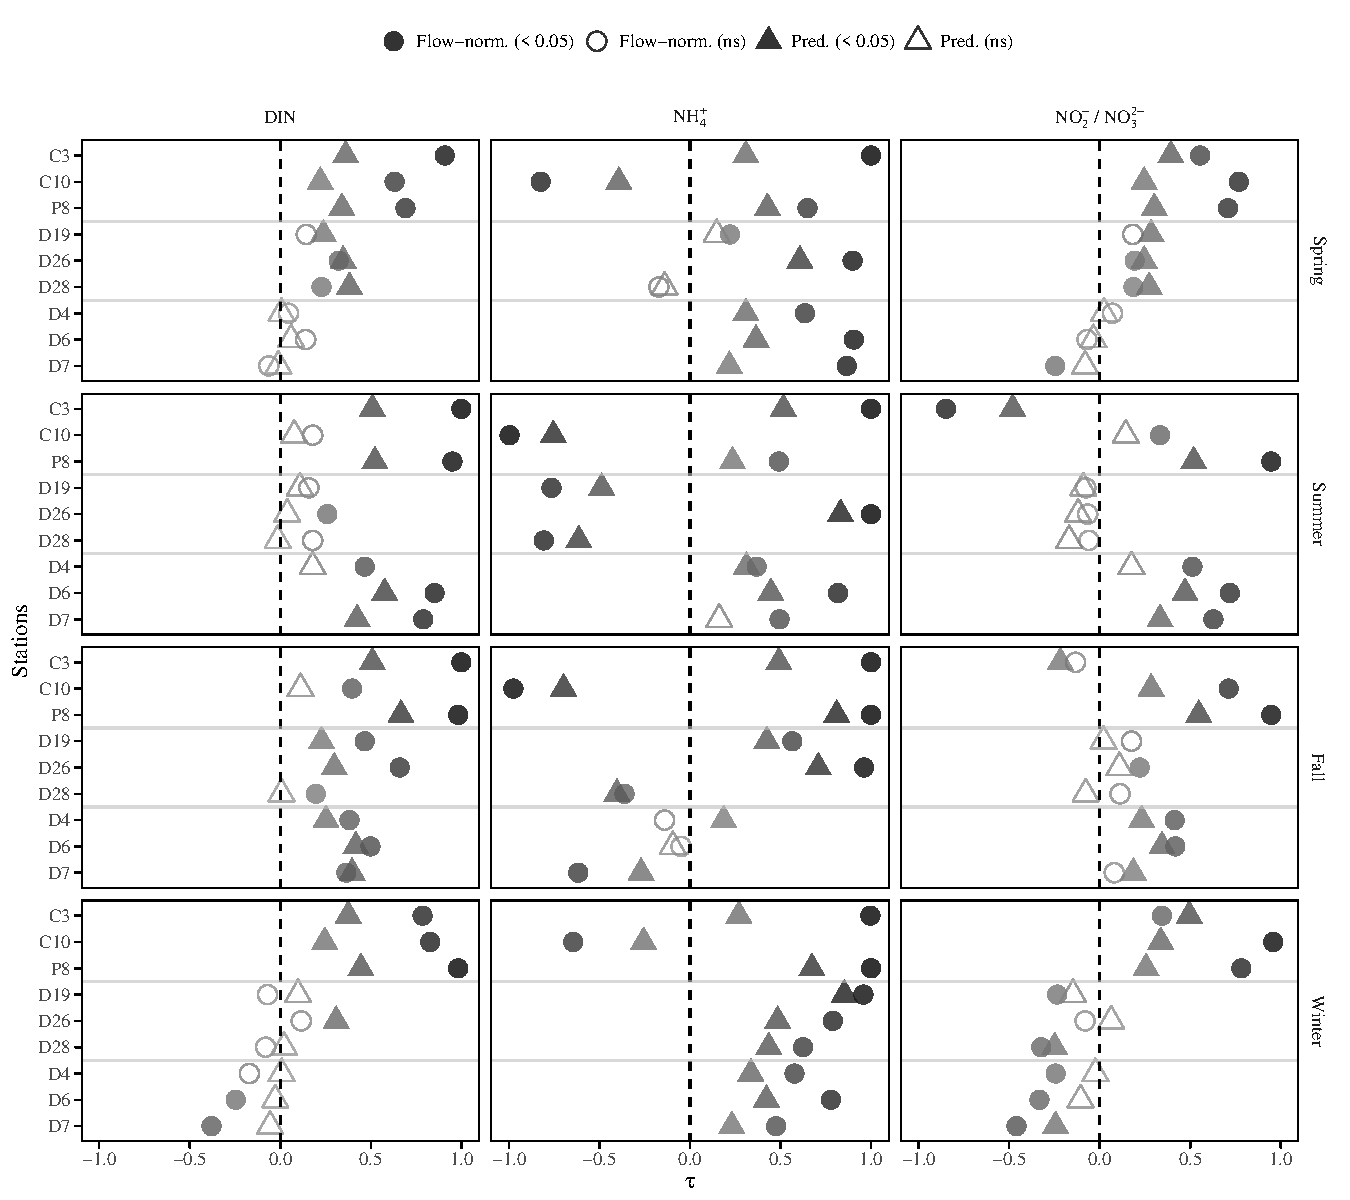
\includegraphics[width=1\textwidth,page=1]{figs/trndcomp2.pdf}
\caption{Results from seasonal Kendall tests on observed data (triangles) and flow-normalized predictions (circles) from \ac{wrtds} for nitrogen analytes. Results are shown as the percent change per year as the estimated Theil-Sen slope divided by the median for a given aggregation period (significance evaluated at $\alpha = 0.05$, based on $\tau$). Trends are shown separately for different seasonal groupings from 1976-1995. Months for each season are Spring: MAM, Summer: JJA, Fall: SON, Winter: DJF. See \cref{fig:trndcomp1} for annual comparisons.}
\label{fig:trndcomp2}   
\end{figure}

\begin{figure}
\centering
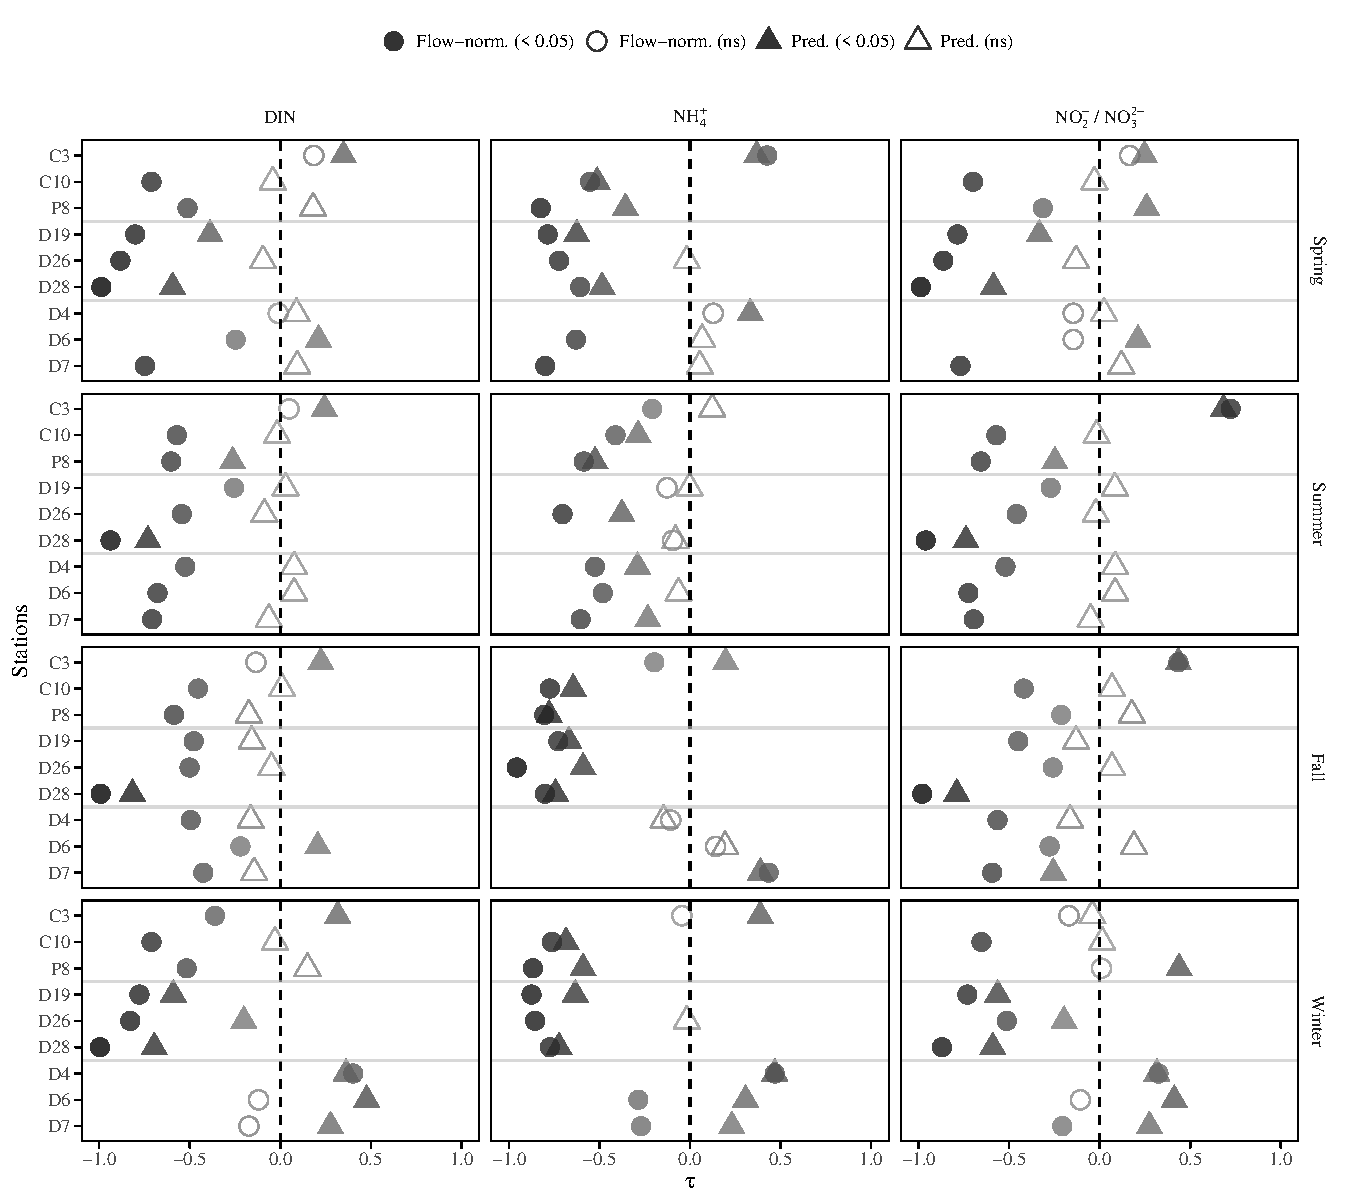
\includegraphics[width=1\textwidth,page=1]{figs/trndcomp3.pdf}
\caption{Results from seasonal Kendall tests on observed data (triangles) and flow-normalized predictions (circles) from \ac{wrtds} for nitrogen analytes. Results are shown as the percent change per year as the estimated Theil-Sen slope divided by the median for a given aggregation period (significance evaluated at $\alpha = 0.05$, based on $\tau$). Trends are shown separately for different seasonal groupings from 1996-2013. Months for each season are Spring: MAM, Summer: JJA, Fall: SON, Winter: DJF. See \cref{fig:trndcomp1} for annual comparisons.}
\label{fig:trndcomp3}   
\end{figure}

\begin{figure}[!ht]

{\centering 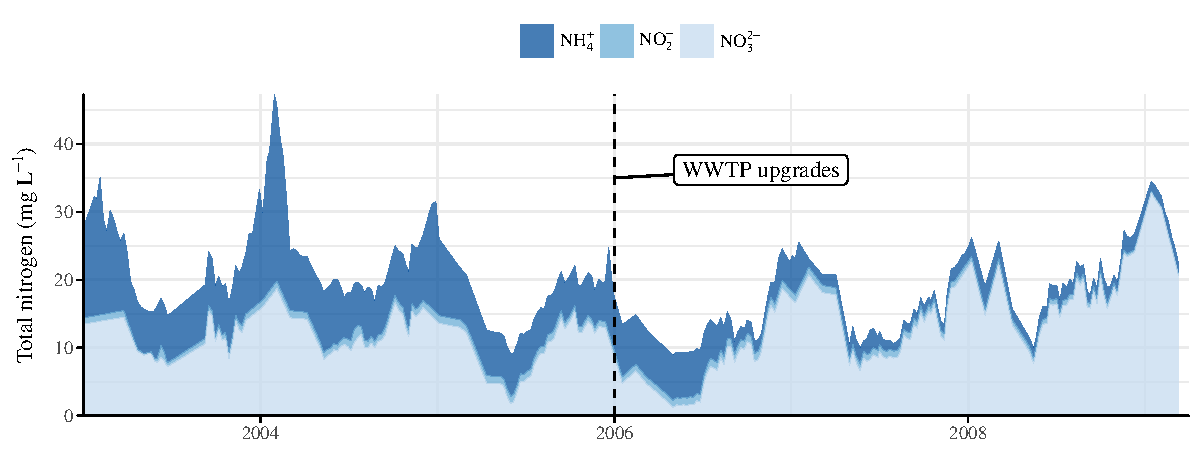
\includegraphics[width=\textwidth]{figs/stock-1} 

}

\caption[Nitrogen concentration measurements (mg L$^{-1}$) from the City of Stockton Wastewater Treatment Plant, San Joaquin County]{Nitrogen concentration measurements (mg L$^{-1}$) from the City of Stockton Wastewater Treatment Plant, San Joaquin County.  Wastewater discharge requirements were implemented in 2006 for nitrification/denitrification and tertiary filtration to convert ammonium to nitrate.}\label{fig:stock}
\end{figure}



\end{suppinfo}

\end{document}
